%% 该模板修改自《计算机学报》latex 模板
%% 主要是将双栏改成单栏,去掉了部分计算机学报标识;
%% 源文件自:https://www.overleaf.com/latex/templates/latextemplet-cjc-xelatex/ybmmymncrrmw
%% 
%%
%% This is file `CjC_template_tex.tex',
%% is modified by Zhi Wang (zhiwang@ieee.org) based on the template 
%% provided by Chinese Journal of Computers (http://cjc.ict.ac.cn/).
%%
%% This version is capable with Overleaf (XeLaTeX).
%%
%% Update date: 2023/03/10
%% -------------------------------------------------------------------
%% Copyright (C) 2016--2023 
%% -------------------------------------------------------------------
%% This file may be distributed and/or modified under the
%% conditions of the LaTeX Project Public License, either version 1.3c
%% of this license or (at your option) any later version.
%% The latest version of this license is in
%%    https://www.latex-project.org/lppl.txt
%% and version 1.3c or later is part of all distributions of LaTeX
%% version 2008 or later.
%% -------------------------------------------------------------------

\documentclass[10.5pt,compsoc,UTF8]{CjC}
\usepackage{CTEX}
\usepackage{graphicx}
\usepackage{footmisc}
\usepackage{subfigure}
\usepackage{url}
\usepackage{multirow}
\usepackage{multicol}
\usepackage[noadjust]{cite}
\usepackage{amsmath,amsthm}
\usepackage{amssymb,amsfonts}
\usepackage{booktabs}
\usepackage{color}
\usepackage{ccaption}
\usepackage{booktabs}
\usepackage{float}
\usepackage{fancyhdr}
\usepackage{caption}
\usepackage{xcolor,stfloats}
\usepackage{comment}
\setcounter{page}{1}
\graphicspath{{figures/}}
\usepackage{cuted}%flushend,
\usepackage{captionhack}
\usepackage{epstopdf}
\usepackage{gbt7714}
\usepackage{listings}
\usepackage{xeCJK}
\usepackage{float}
\usepackage{sourcecodepro}
\usepackage[T1]{fontenc}
\usepackage{hyperref}

\setmainfont{Times Roman}
% \setCJKmainfont{Noto Sans Mono CJK TC}
\setCJKmainfont{標楷體.ttc}
\setmonofont{Cascadia Code}

%===============================%

\headevenname{\mbox{\quad} \hfill  \mbox{\zihao{-5}{ \hfill 2024 Hardware Design  } \hspace {50mm} \mbox{2024 年 9 月}}}%
\headoddname{Group 21 \hfill Lab 2: Advanced Gate-Level Verilog}%

%footnote use of *
\renewcommand{\thefootnote}{\fnsymbol{footnote}}
\setcounter{footnote}{0}
\renewcommand\footnotelayout{\zihao{5-}}

\newtheoremstyle{mystyle}{0pt}{0pt}{\normalfont}{1em}{\bf}{}{1em}{}
\theoremstyle{mystyle}
\renewcommand\figurename{figure~}
\renewcommand{\thesubfigure}{(\alph{subfigure})}
\newcommand{\upcite}[1]{\textsuperscript{\cite{#1}}}
\renewcommand{\labelenumi}{(\arabic{enumi})}
\newcommand{\tabincell}[2]{\begin{tabular}{@{}#1@{}}#2\end{tabular}}
\newcommand{\abc}{\color{white}\vrule width 2pt}
\renewcommand{\bibsection}{}
\makeatletter
\renewcommand{\@biblabel}[1]{[#1]\hfill}
\makeatother
\setlength\parindent{2em}
%\renewcommand{\hth}{\begin{CJK*}{UTF8}{gbsn}}
%\renewcommand{\htss}{\begin{CJK*}{UTF8}{gbsn}}
\renewcommand{\contentsname}{Table of Contents}


\begin{document}

\hyphenpenalty=50000
\makeatletter
\newcommand\mysmall{\@setfontsize\mysmall{7}{9.5}}
\newenvironment{tablehere}
  {\def\@captype{table}}

\let\temp\footnote
\renewcommand \footnote[1]{\temp{\zihao{-5}#1}}

\hypersetup{
  colorlinks=false,
  pdfborder={0 0 0},
}

\thispagestyle{plain}%
\thispagestyle{empty}%
\pagestyle{CjCheadings}

% \begin{table*}[!t]
\vspace {-13mm}


\onecolumn
\zihao{5-}\noindent Group 21 \hfill Lab 2: Advanced Gate-Level Verilog \hfill 2024 年 9 月\\
\noindent\rule[0.25\baselineskip]{\textwidth}{1pt}


\begin{center}
    \vspace {11mm}
    {\zihao{2} \heiti \fangsong Lab 2: Advanced Gate-Level Verilog }
    
    \vskip 5mm
    
    {\zihao{4}\fangsong Group 21: 陳克盈(112062205)、蔡明妡(112062224)}
\end{center}

\lstset{
    % backgroundcolor=\color{red!50!green!50!blue!50},%程式碼塊背景色為淺灰色
    rulesepcolor= \color{gray}, %程式碼塊邊框顏色
    breaklines=true,  %程式碼過長則換行
    numbers=left, %行號在左側顯示
    numberstyle= \small\ttfamily,%行號字型
    keywordstyle= \color{blue},%關鍵字顏色
    commentstyle=\color{gray}, %註釋顏色
    frame=shadowbox%用方框框住程式碼塊
    basicstyle=\ttfamily\footnotesize,
}
 
\definecolor{improvecolor}{rgb}{0,0.6,0} % 深綠色
\definecolor{declinecolor}{rgb}{0.6,0,0} % 深紅色


%%%%%%%%%%%%%%%%%%%%%%%%%%%%%%%%%%%%%%
\zihao{5}
\vskip 10mm
% \begin{multicols}{1}


%%%%%%%%%%%%%%%%%%%%%%%%%%%%%%%%%%%%%%%%%%
%%%%%%%%%%%%%%%%%%%%%%%%%%%%%%%%%%%%%%%%%%

\tableofcontents
\newpage

\section{Q0: Basic Questions}
\label{sec:NAND Gate to all other gates}
在 Basic Questions 中,需要使用 NAND Gate 實現出所有的基本邏輯閘,\
並透過 $sel$ 的數值來控制要輸出哪一種邏輯閘的結果,$sel$ 與要求的輸出可以參考圖 \ref{fig:Basic Q1 spec}。

\begin{figure}[htp]
  \centering
  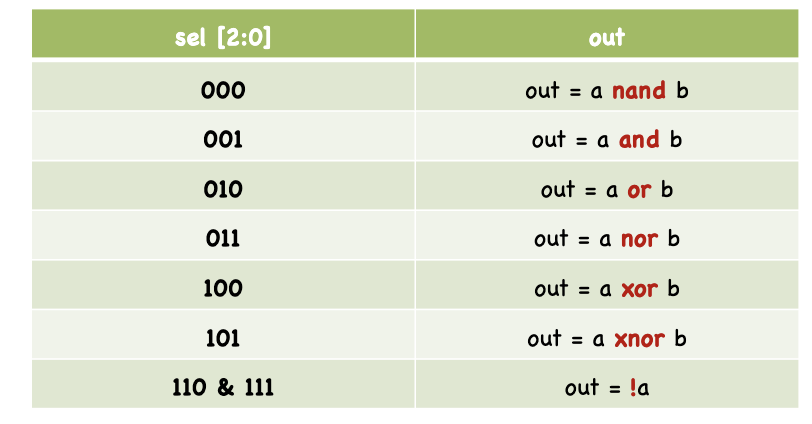
\includegraphics[width=0.8\textwidth]{Basic-Q1-spec.png}
  \caption{Basic Q1 spec}
  \label{fig:Basic Q1 spec}
\end{figure}
\subsection{NAND Gate to all other gates}

NAND 之所以被稱為 Universal Gate,是因為他能夠生成出所有其他的邏輯閘,\
而這正是 Basic Questions 的核心。圖 \ref{fig:NAND to all other gates} 演示了如何使用 NAND Gate 實現的所有基本邏輯閘。
\par
此章節利用 NAND 所組成的所有邏輯閘,都將用來作為後續所有題目的邏輯閘使用。\
不過在表示上為求可讀性,將會使用一般的邏輯閘符號來表示。

\begin{figure}[htp]
  \centering
  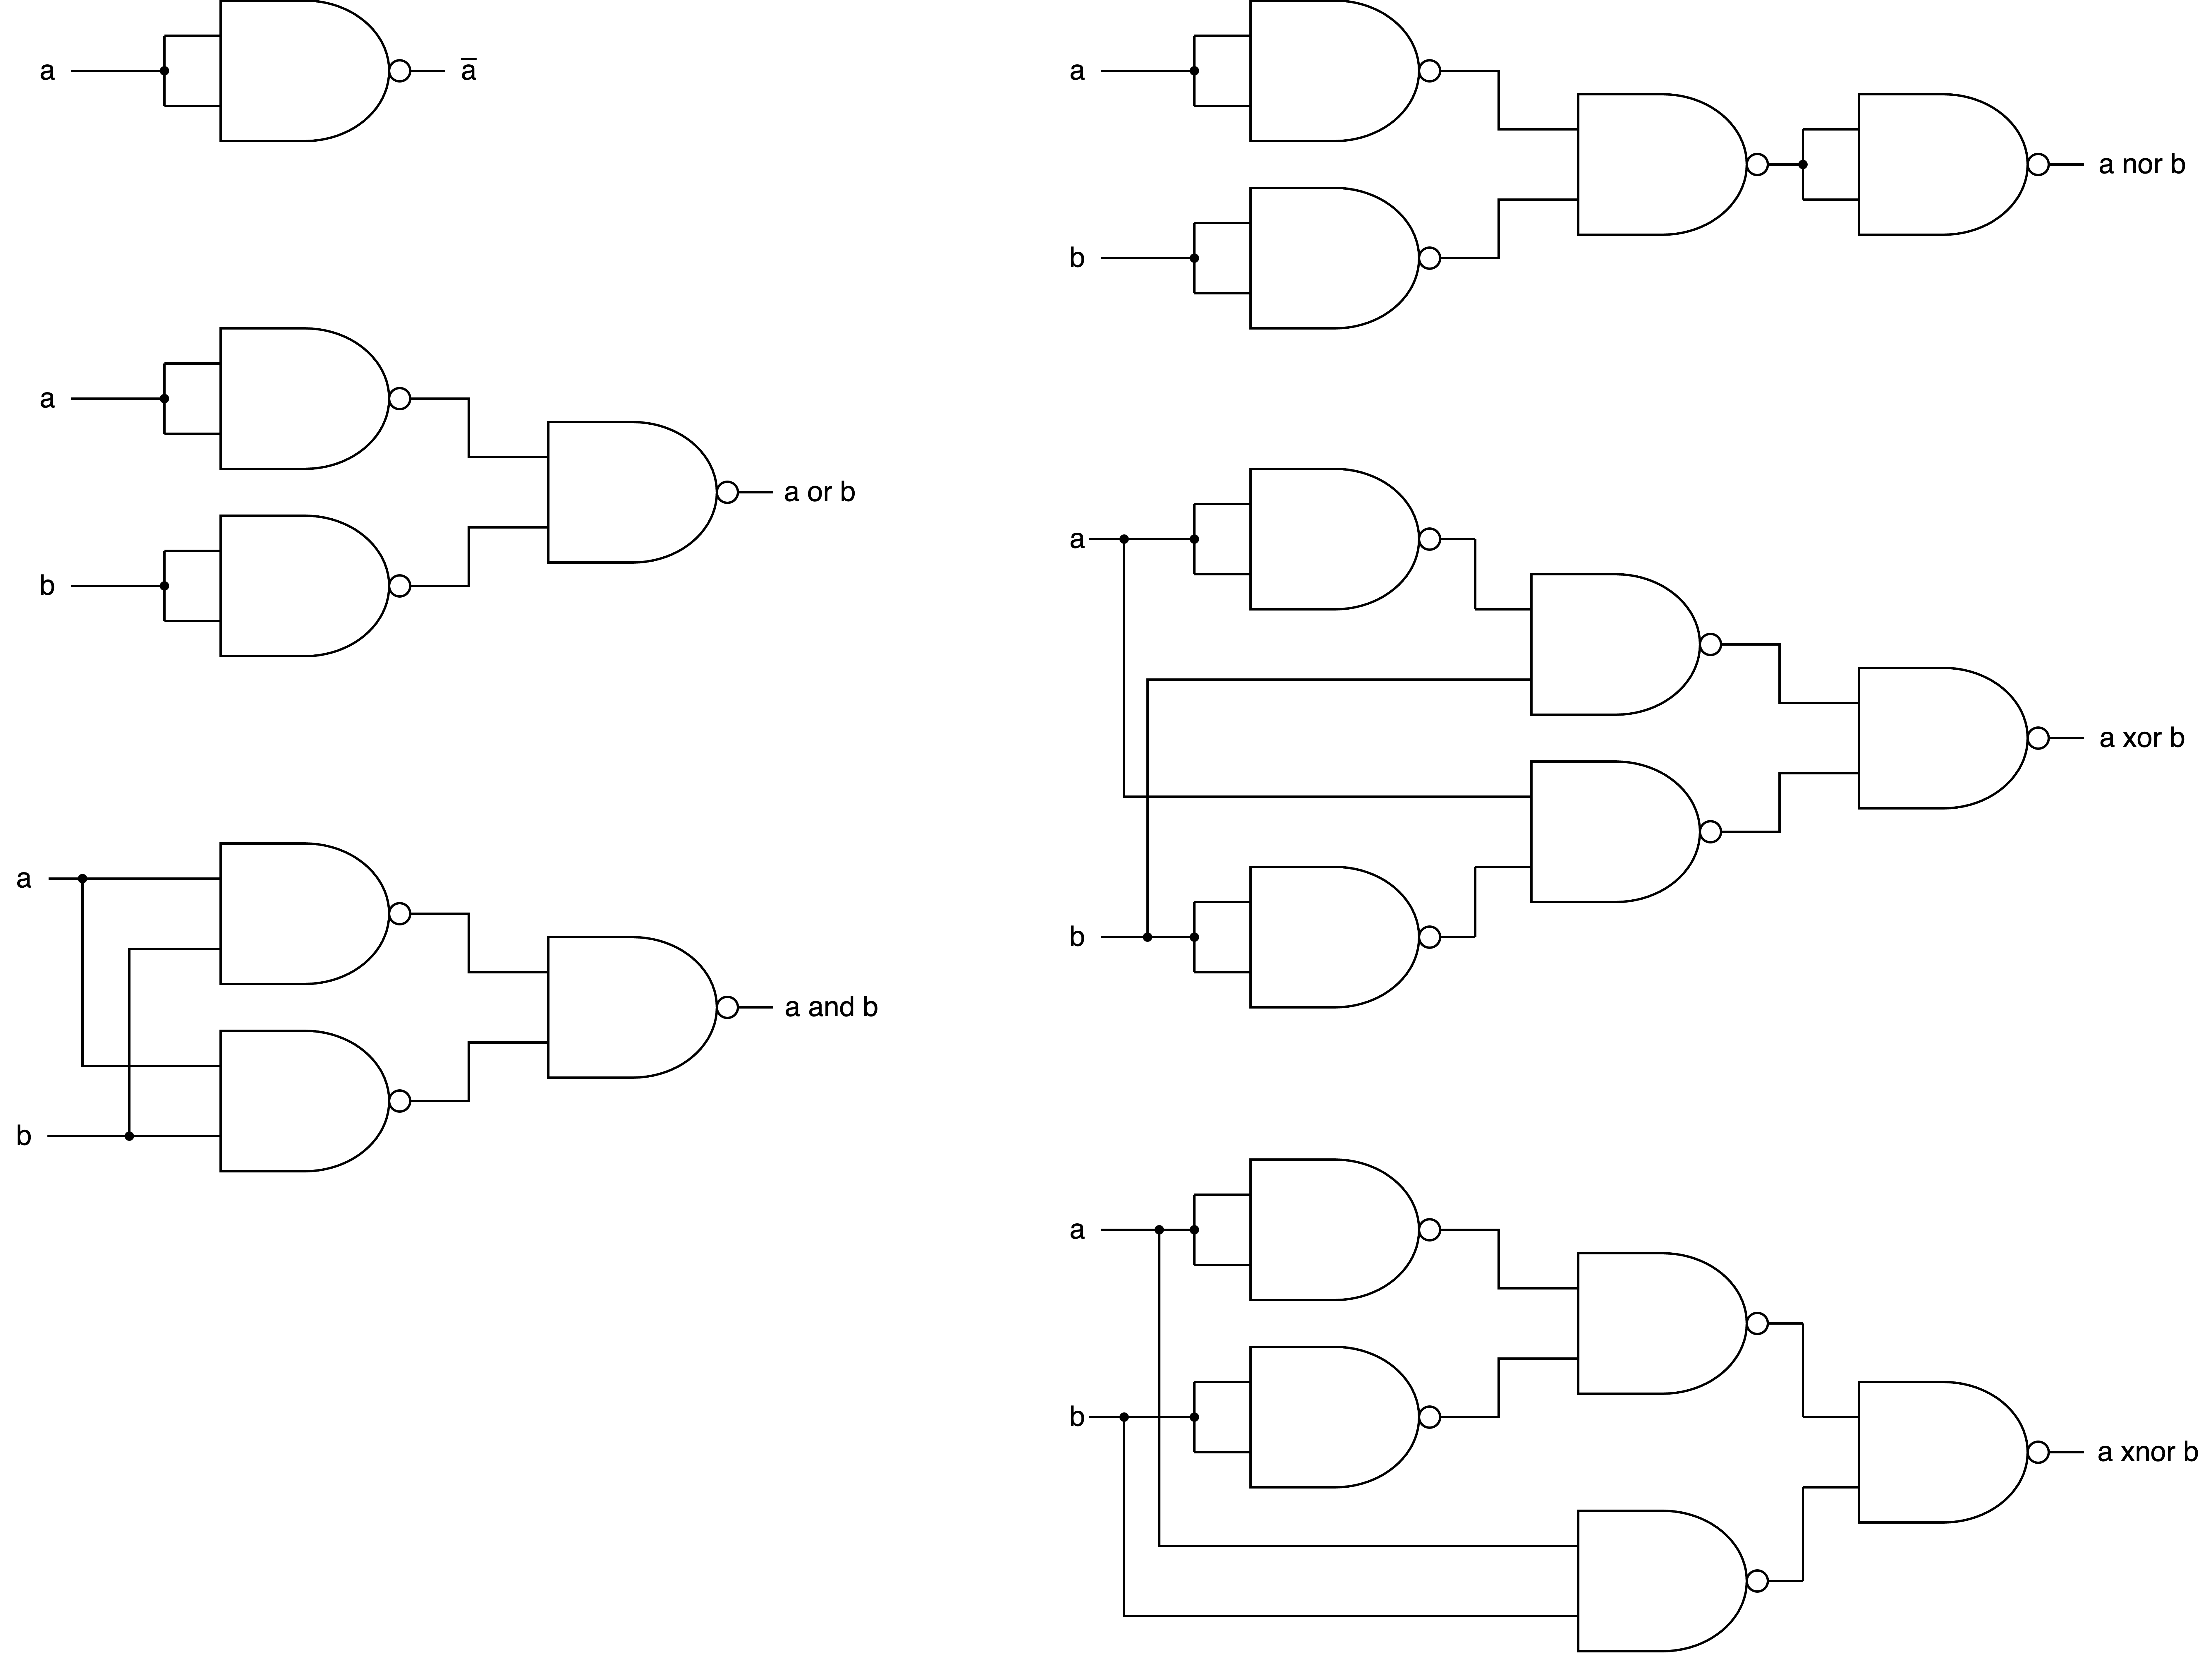
\includegraphics[width=\textwidth]{gates.png}
  \caption{NAND to all other gates}
  \label{fig:NAND to all other gates}
\end{figure}

\subsubsection*{Decoder}

我們使用了圖 \ref{fig:2-to-1-MUX} 中的 2-to-1 MUX,透過樹狀分治的概念,\
來實現 8-to-1 MUX,而 $A \sim H$ 分別代表了 $sel\ 0 \sim 7$ 對應到邏輯閘的輸出。\
若是將那些 MUX 看成是一個整體,加上 Execute 的部分後就會如圖 \ref{fig:Q0-Decoder} 所示。



\begin{figure}[htp]
  \centering
  
\includegraphics[width=0.4\textwidth]{2-to-1-MUX.png}
  \caption{2-to-1 MUX}
  \label{fig:2-to-1-MUX} 
\end{figure}

\begin{figure}[htp]
  \centering
  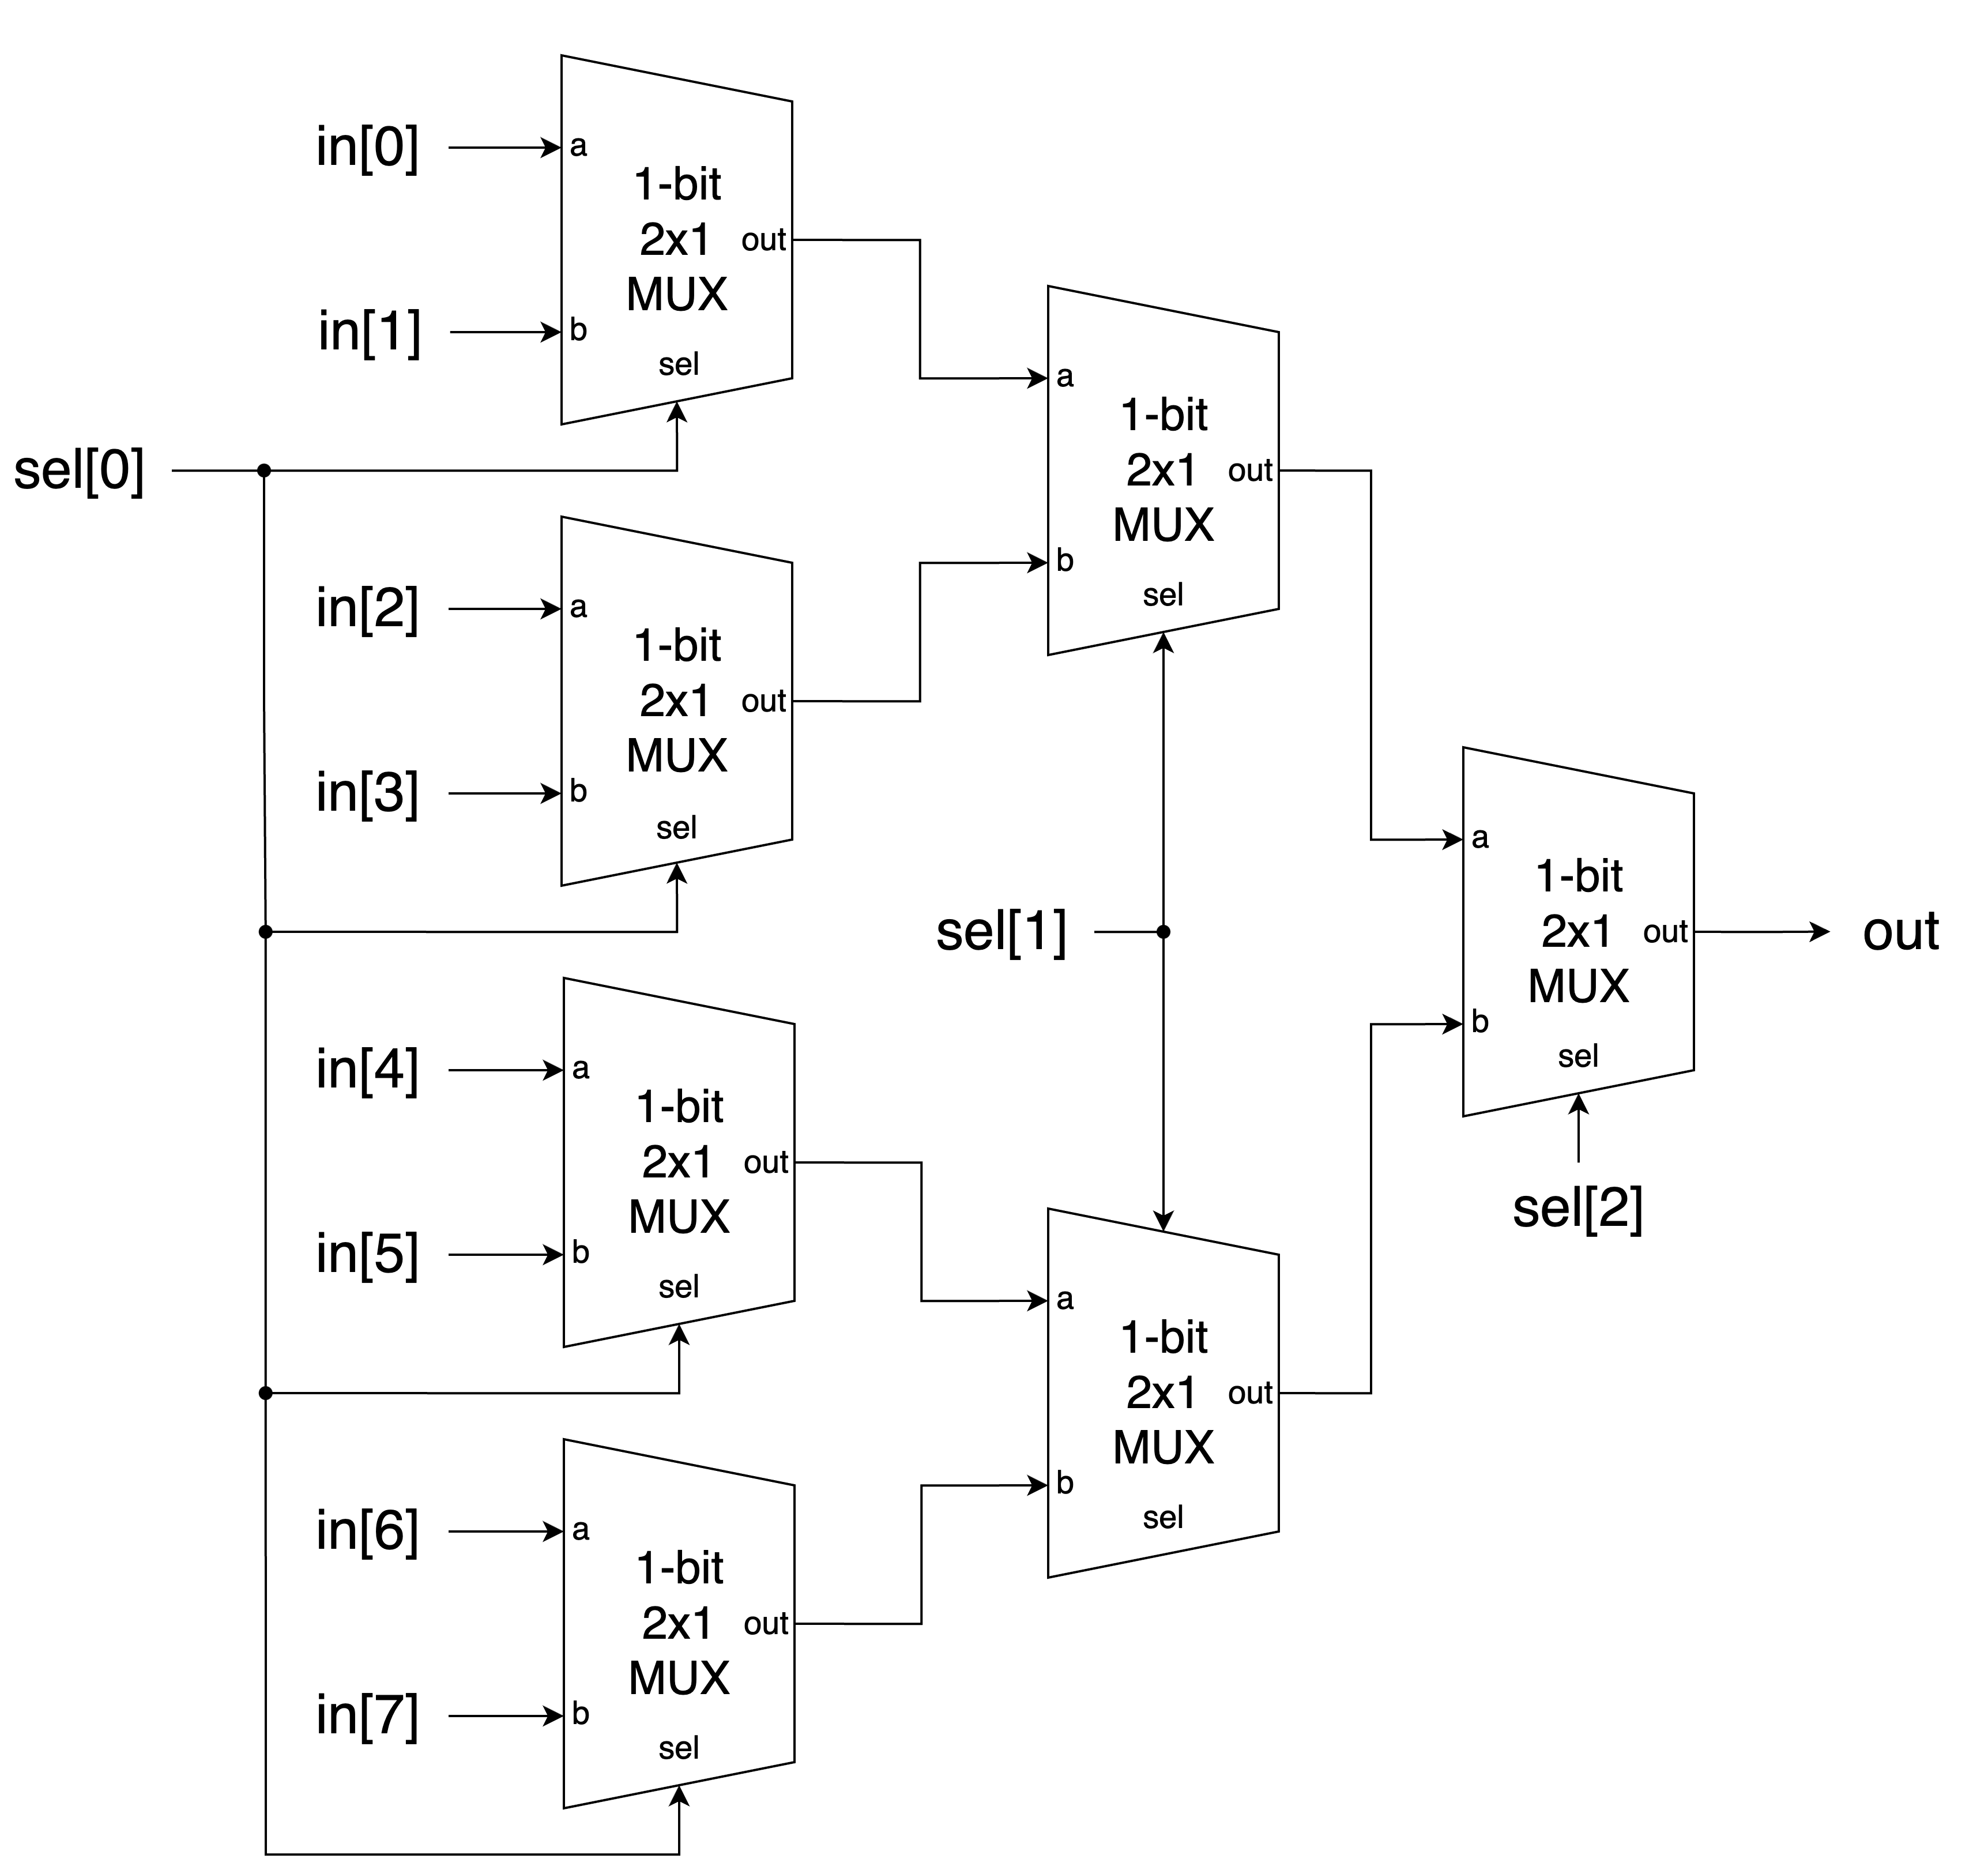
\includegraphics[width=0.8\textwidth]{MUXs.png}
  \caption{8-to-1 MUX}
  \label{fig:2-to-1-MUX} 
\end{figure}

\begin{figure}[htp]
  \centering
  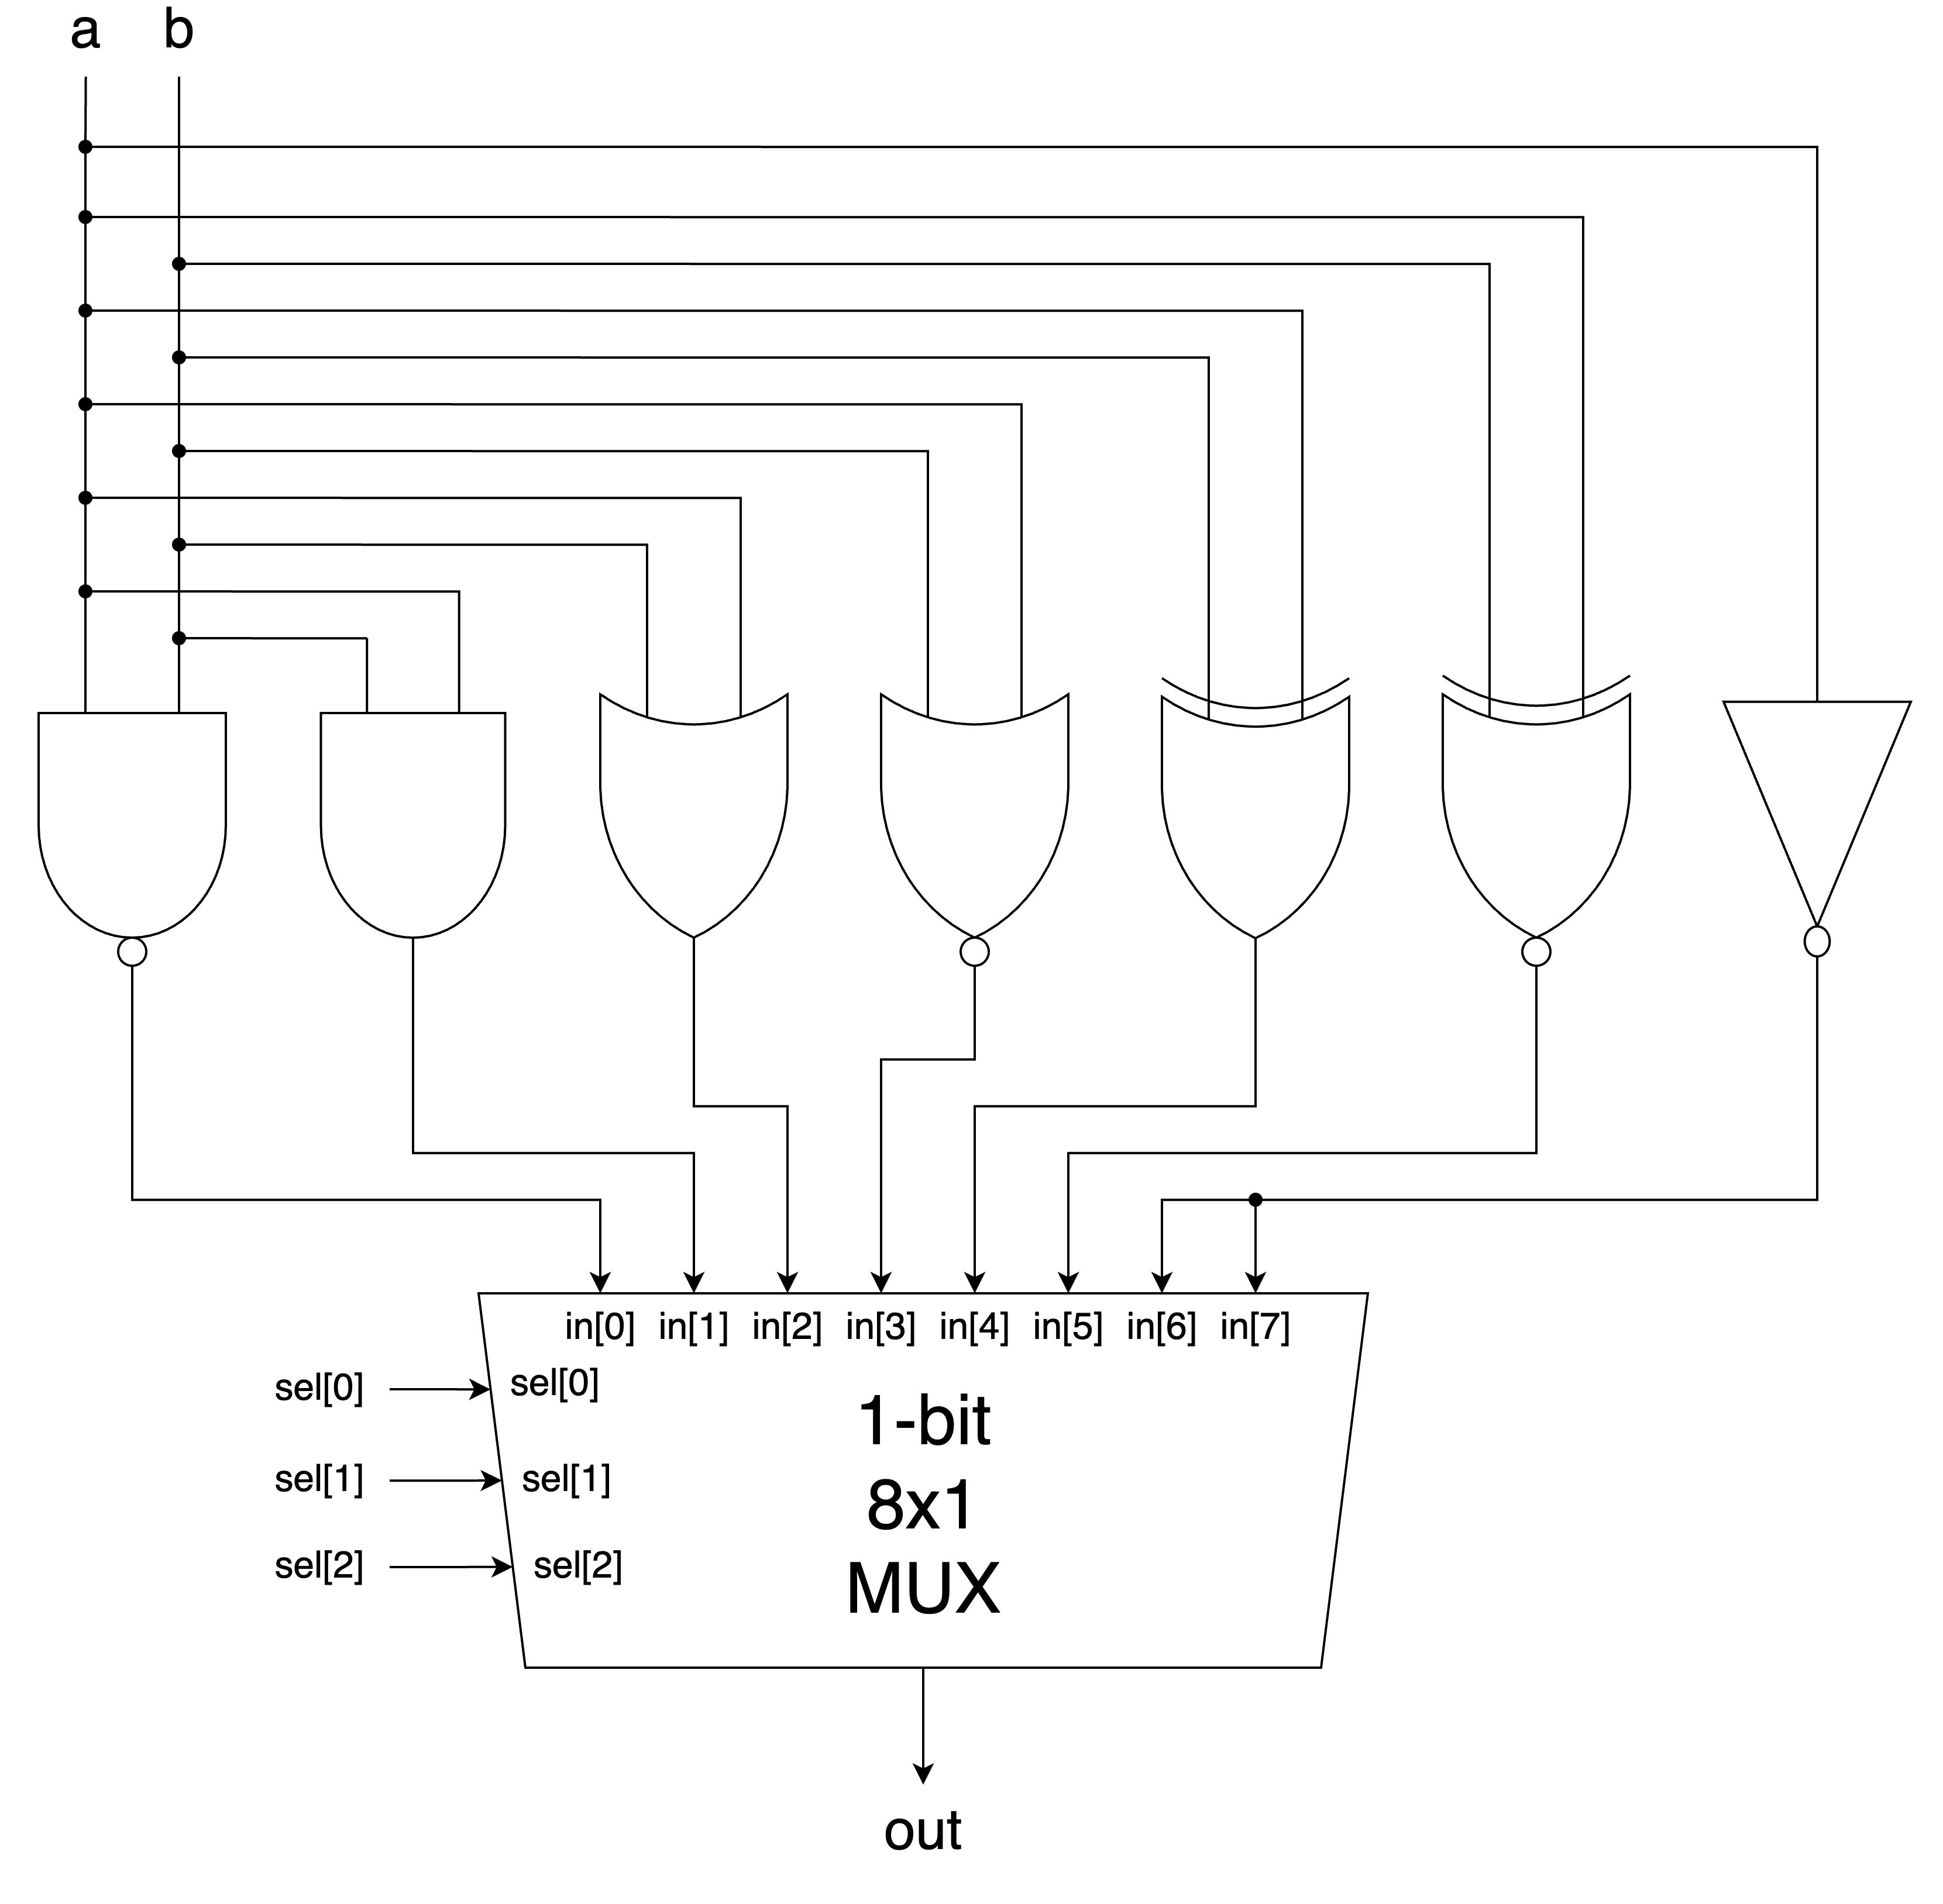
\includegraphics[width=0.5\textwidth]{8-to-1-MUX.png}
  \caption{Decoder}
  \label{fig:Q0-Decoder}
\end{figure}

\newpage

\subsection{Full Adder vs. Half Adder}

在 Basic 中,我們首先使用 NAND Gate 實現了一個 Majority(圖 \ref{fig:Majority}),用來輸出三個參數中,是否有至少兩個參數為 True,以及一個 Half Adder\
,接著將 Majority 與 Half Adder 合併起來就完成了 Full Adder,如圖 \ref{fig:Half-Full Adder} 所示。

\begin{figure}[htp]
  \centering
  
\includegraphics[width=0.4\textwidth]{Majority.png}
  \caption{Majority Circuit}
  \label{fig:Majority}
\end{figure}
\par

圖\ref{fig:Half-Full Adder} 為兩者的電路圖,兩者差異在於,Half Adder 雖然能夠算出總和以及進位值,但由於缺少了 $cin$  的輸入,\
導致他只能處理單一位元的加法,並且也不需要使用 Majority 來判定 $cout$,這也是為什麼他被稱作是 Half Adder。
\begin{figure}[htp]
  \centering
  
\includegraphics[width=0.4\textwidth]{Half-Adder.png}
  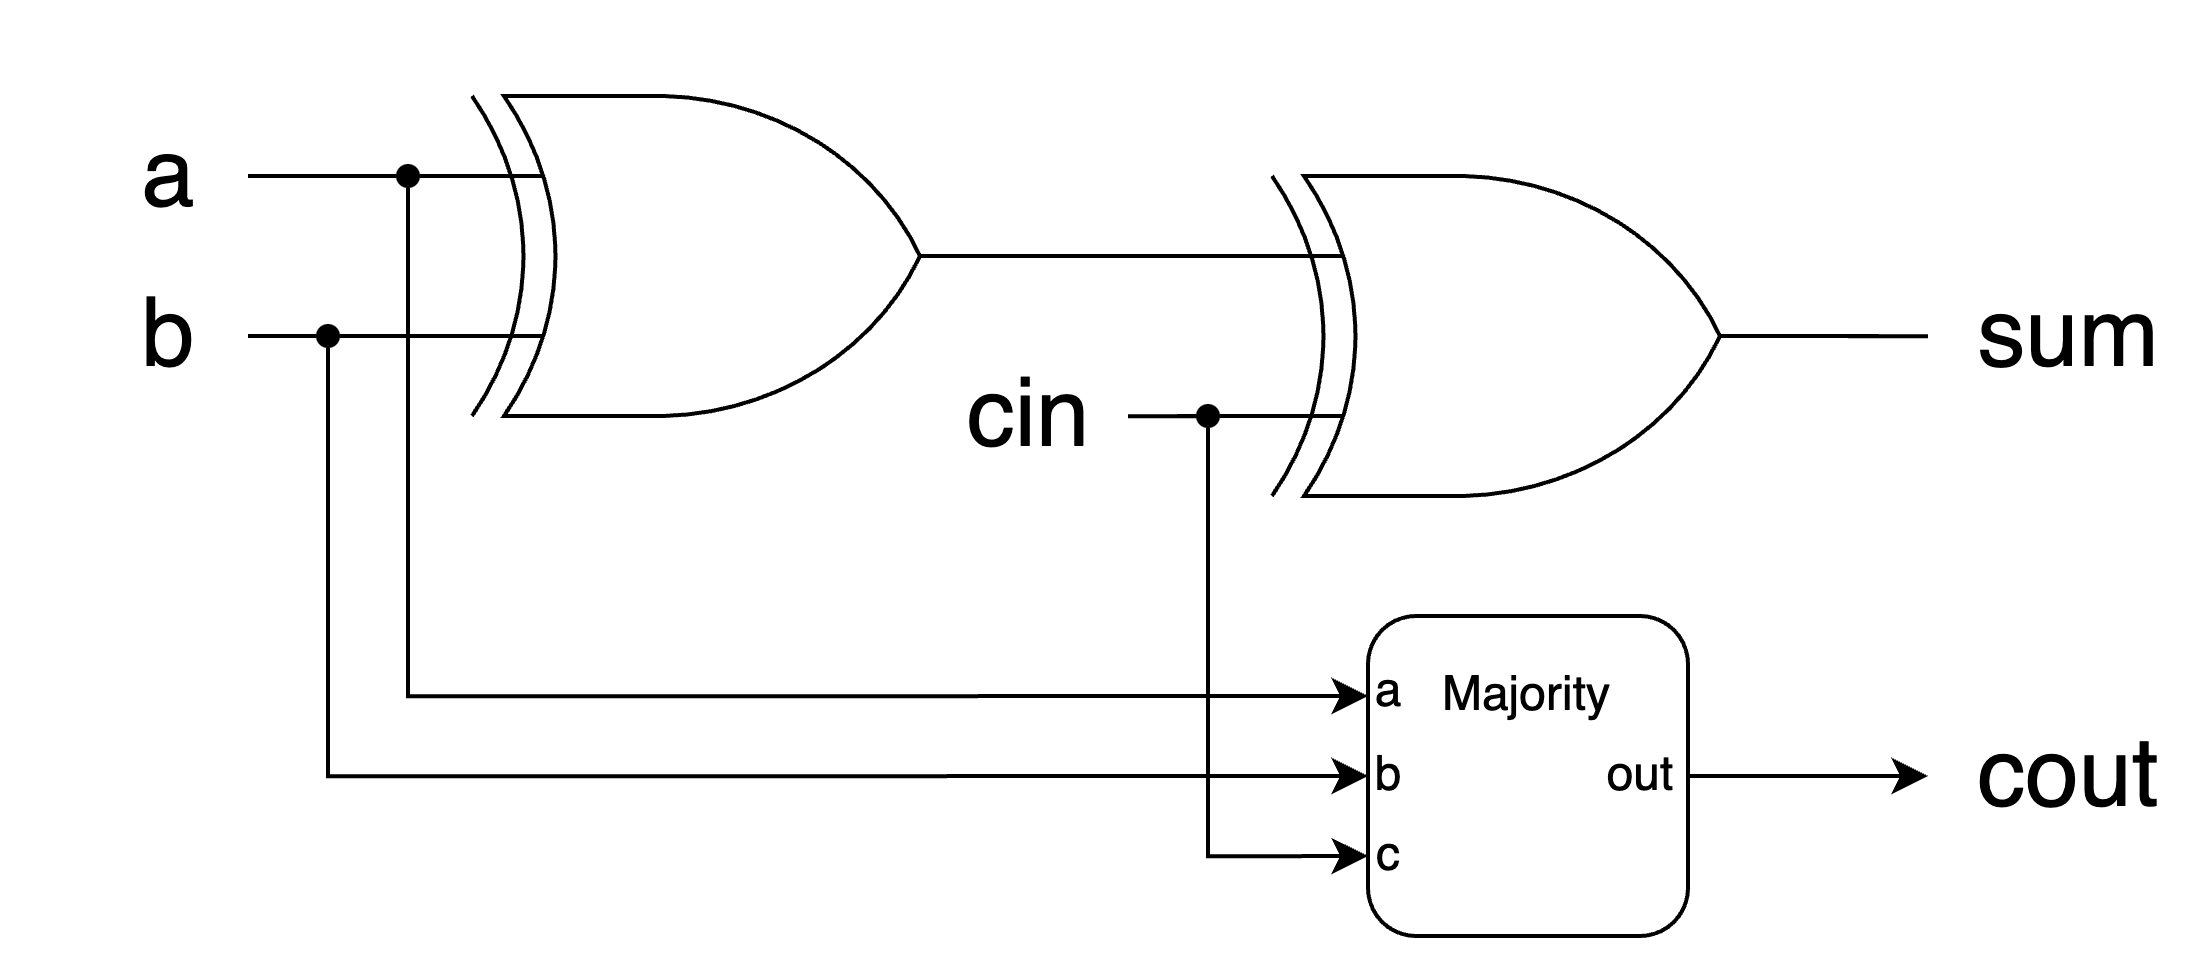
\includegraphics[width=0.4\textwidth]{Full-Adder.png}
  \caption{Half Adder (left) and Full Adder (right)}
  \label{fig:Half-Full Adder}
\end{figure}

\newpage

\section{Q1: 8-bit ripple carry adder}
\label{sec:Q1}

\subsection{Implement \& Circuit}

題目所求(參考附圖 \ref{fig:Q1_spec})為建立一個 8-bit 的 Ripple Carry Adder。我們使用 8 個上個章節提到的\
Full Adder,將他們依據順序將輸入輸出串接在一起,便完成了題目所求(圖 \ref{fig:Q1_circuit})。

\begin{figure}[htp]
  \centering
  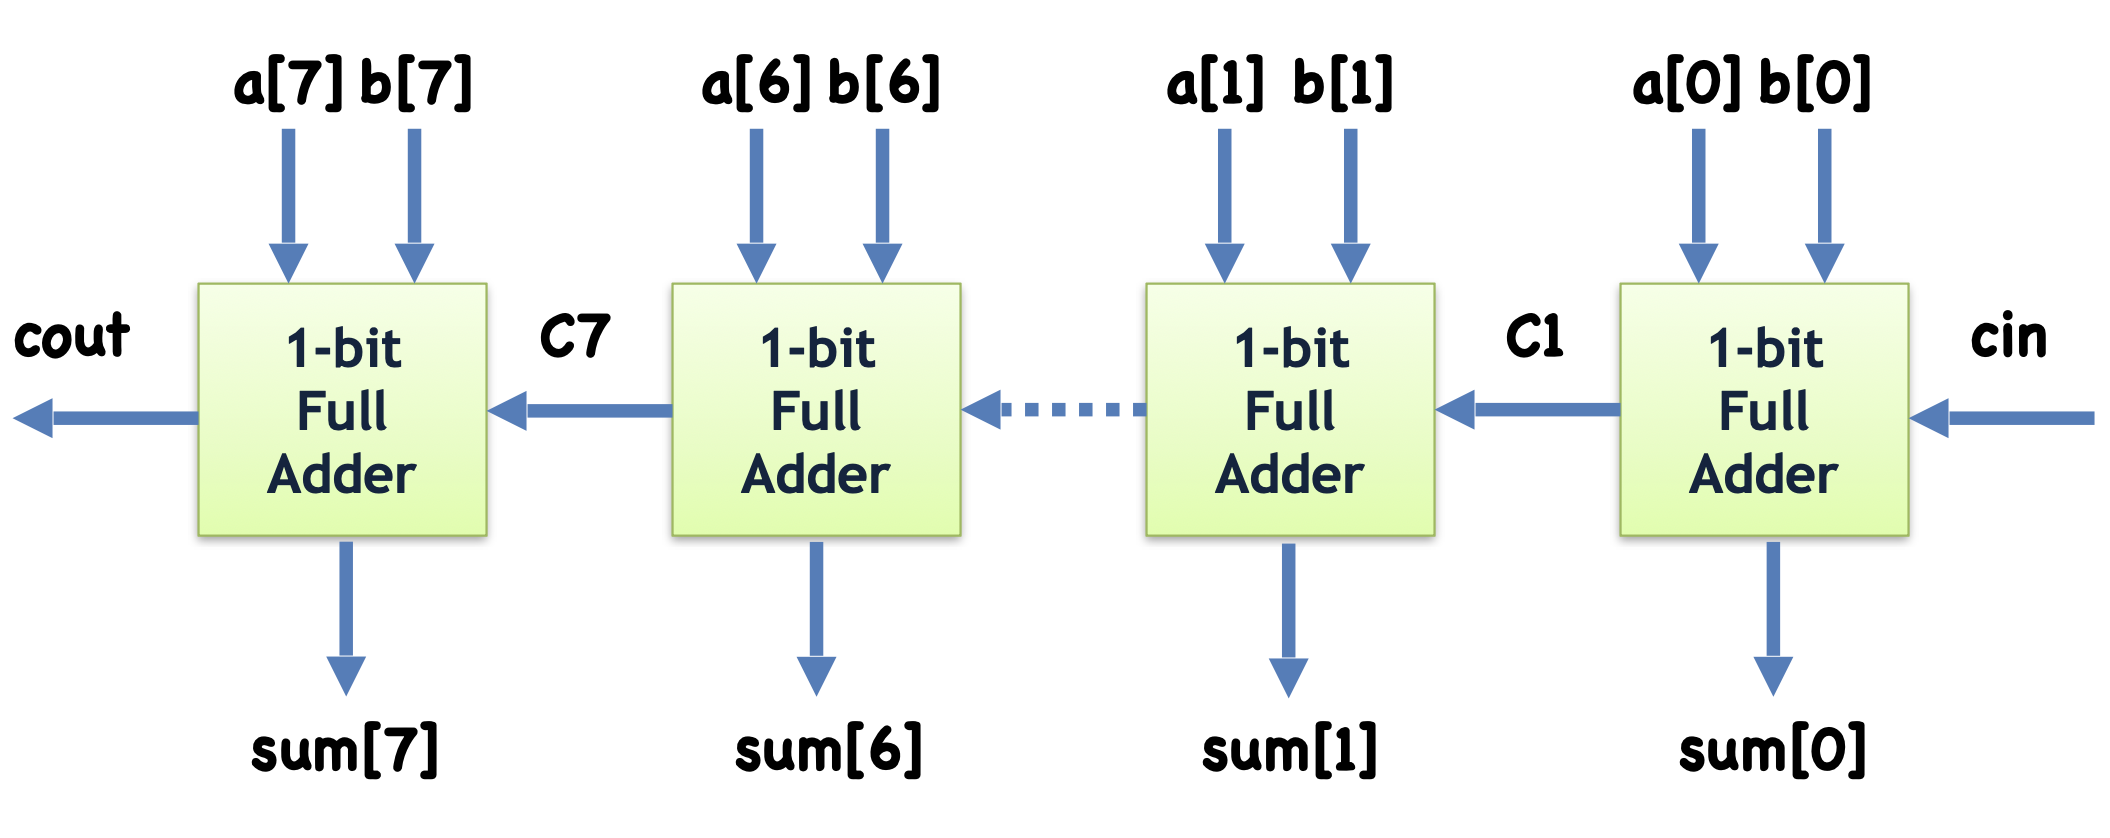
\includegraphics[width=0.8\textwidth]{Q1_spec.png}
  \caption{8-bit ripple carry adder spec}
  \label{fig:Q1_spec}
\end{figure}

\begin{figure}[htp]
  \centering
  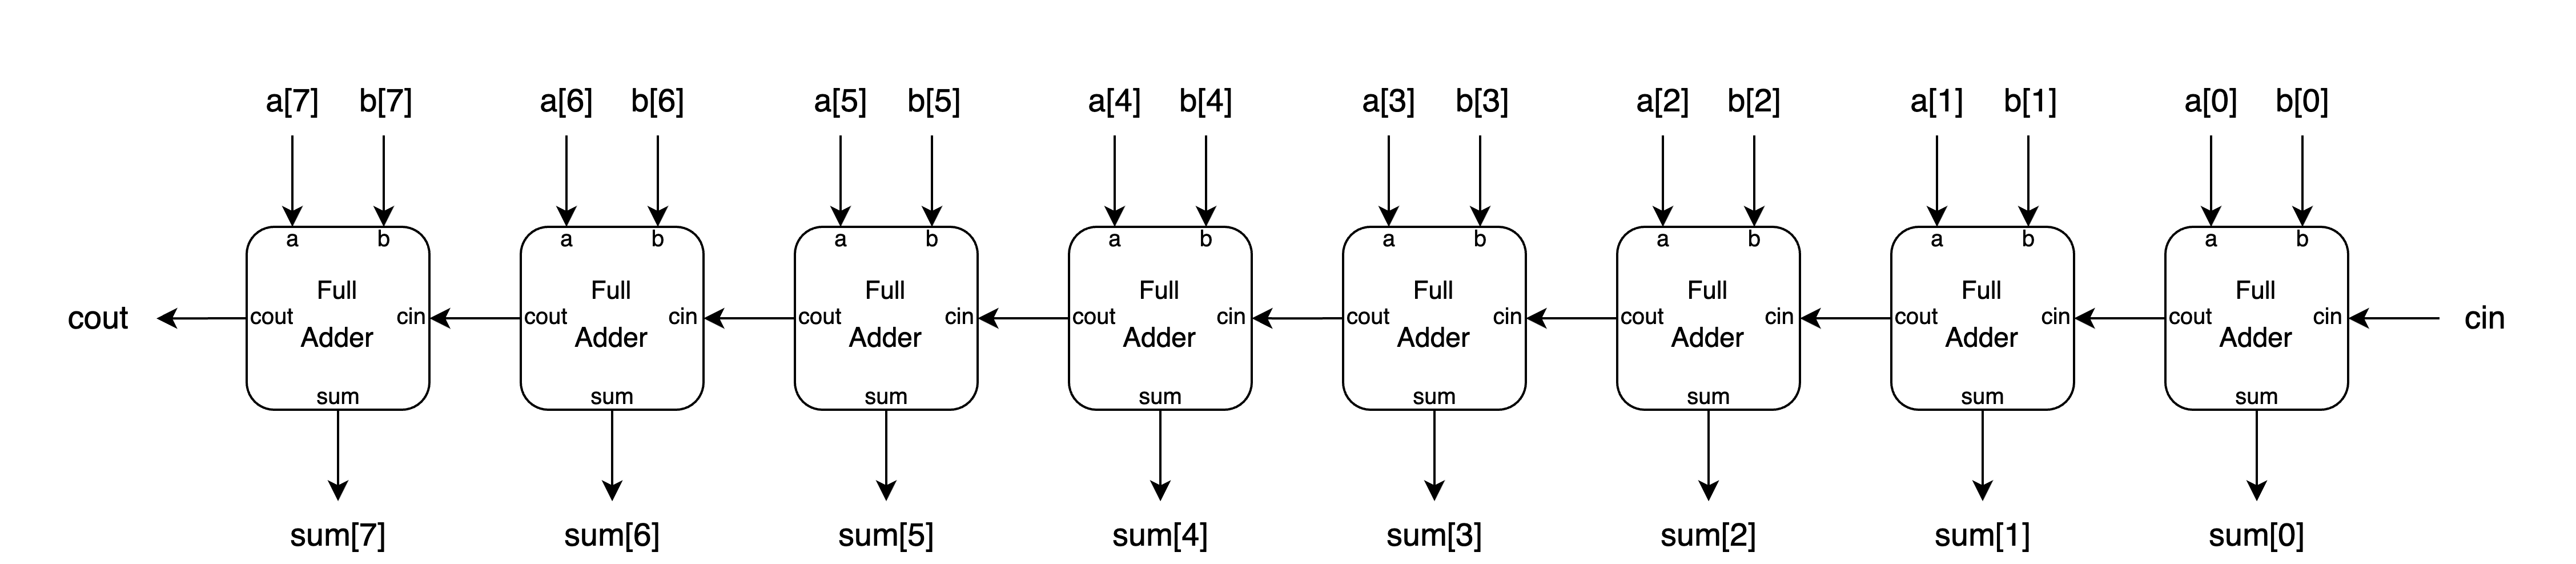
\includegraphics[width=\textwidth]{Adders.png} 
  \caption{8-bit ripple carry adder}
  \label{fig:Q1_circuit} 
\end{figure}



\subsection{Testbench}
\label{sec:Q1_testbench}
我們試著將 $a, b, cin$ 的 $2^{17}$ 種可能全部模擬過一次,但是發現由於 vivado 預設模擬時長的緣故,無法跑完完整的 $131072$ 次模擬,\
將模擬時長調大後便能夠成功完整的模擬所有可能,模擬結果如圖(\ref{fig:Q1_wave})。

\begin{figure}[h]
  \centering
  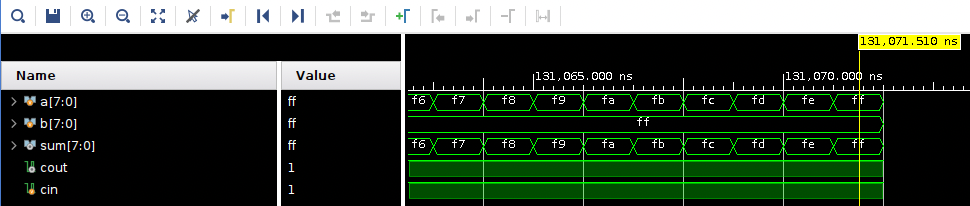
\includegraphics[width=0.8\textwidth]{Q1-wave.png}
  \caption{Q1 testbench wave}
  \label{fig:Q1_wave}
\end{figure}

但是這麼多可能實在是無法用肉眼檢查,因此我們搭配了 verilog 的 if statement,只要遇到 $sum \neq a + b + cin$ 的情況,\
就直接結束模擬,程式碼如圖 \ref{fig:Q1_tb}。上圖有成功跑完所有模擬,代表著沒有出現錯誤。

\begin{figure}[h]
  \centering
  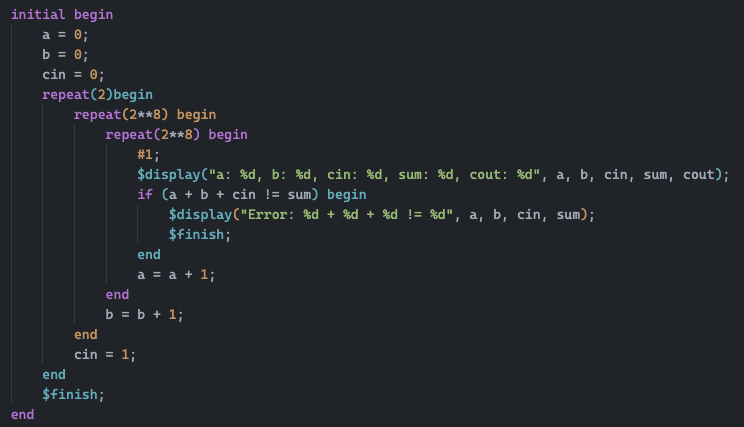
\includegraphics[width=0.8\textwidth]{Q1-tb.png}
  \caption{Q1 testbench code}
  \label{fig:Q1_tb}
\end{figure}

\newpage

\section{Q2: Decode and execute}
\label{sec:Q2}
此題給了一個 Universal Gate,要求使用這個 Gate 實作出其他基本邏輯閘,\
並使用這些邏輯閘實作出一個 Executor 與 Decoder。
\par
其中,Decoder 會收到一個 3-bit 的 $OP\_Code$,我們需要根據 $OP\_Code$ 的不同,\
依據圖 \ref{fig:Q2-spec} 的規定,實作並輸出對應的 Instruction 結果。

\begin{figure}[h]
  \centering
  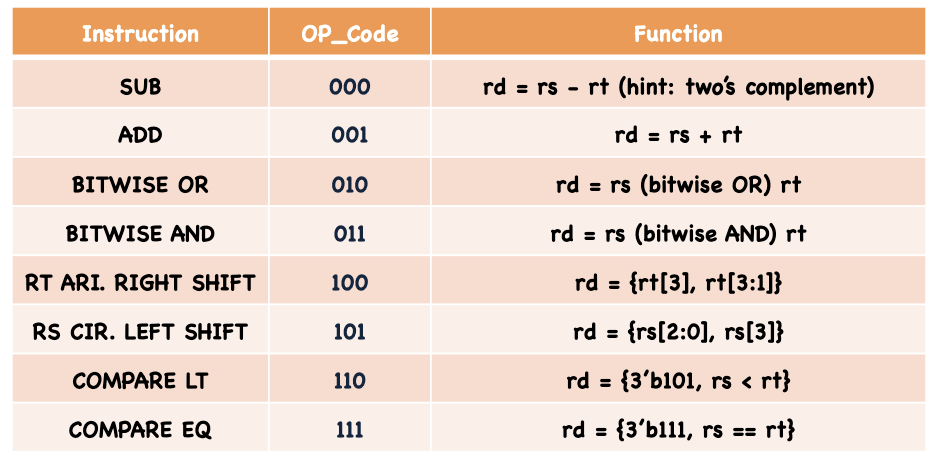
\includegraphics[width=0.6\textwidth]{Q2-spec.png}
  \caption{Q2 spec}
  \label{fig:Q2-spec}
\end{figure}


\subsection{Universal gate}
Universal gate 由 $a \& !b$ 組成,不難發現,當我們將 $a$ 接上 True 信號,\
那麼這個 Gate 就會變成一個 NOT Gate(圖 \ref{fig:Universal Gate})。再利用這個 NOT Gate 接到 $b$ 上,\
就變成了一個 AND Gate。最後,將這個 NOT Gate 接到 AND Gate 的輸出上,\
就完成了一個 NAND Gate,如圖 \ref{fig:Universal Gate to NAND}。

\begin{figure}[h]
  \centering
  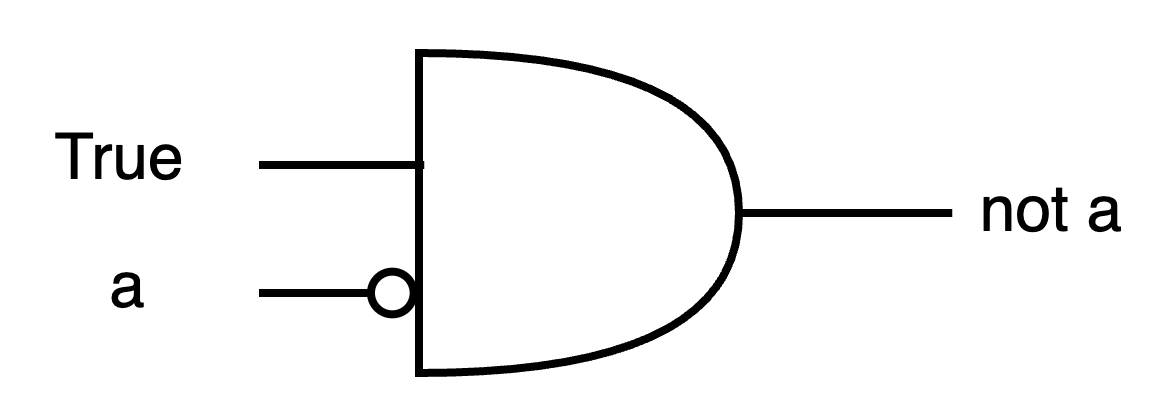
\includegraphics[width=0.4\textwidth]{Universal_not.png}
  \caption{Universal Gate to NOT Gate}
  \label{fig:Universal Gate}
\end{figure}


\begin{figure}[h]
  \centering
  
\includegraphics[width=0.8\textwidth]{Universal_nand.png}
  \caption{Universal Gate to NAND Gate}
  \label{fig:Universal Gate to NAND}
\end{figure}

剩下的所有基本邏輯閘都可以透過這個生成出來的 NAND Gate 組合出來。\
由於是先組成 NAND,而 NAND 的組合方法已經在章節\ref{sec:NAND Gate to all other gates}中提到,\
所有設計皆可直接套用此版本,因此這裡就不再贅述。
\subsection{Executor}
\subsubsection*{SUB}
首先,$rs - rt$ 可以被轉換為 $rs + (-rt)$,根據二補數的規則,可以再轉換為 $rs + \sim rt + 1$。\
再搭配章節\ref{sec:Q1}實現的加法器,改變成 $4-bit Adder$ 後,將 $(a, b, cin)$ 設為 $rs, \sim rt, 1$,便是 SUB 的實現。

\begin{figure}[htp]
  \centering
  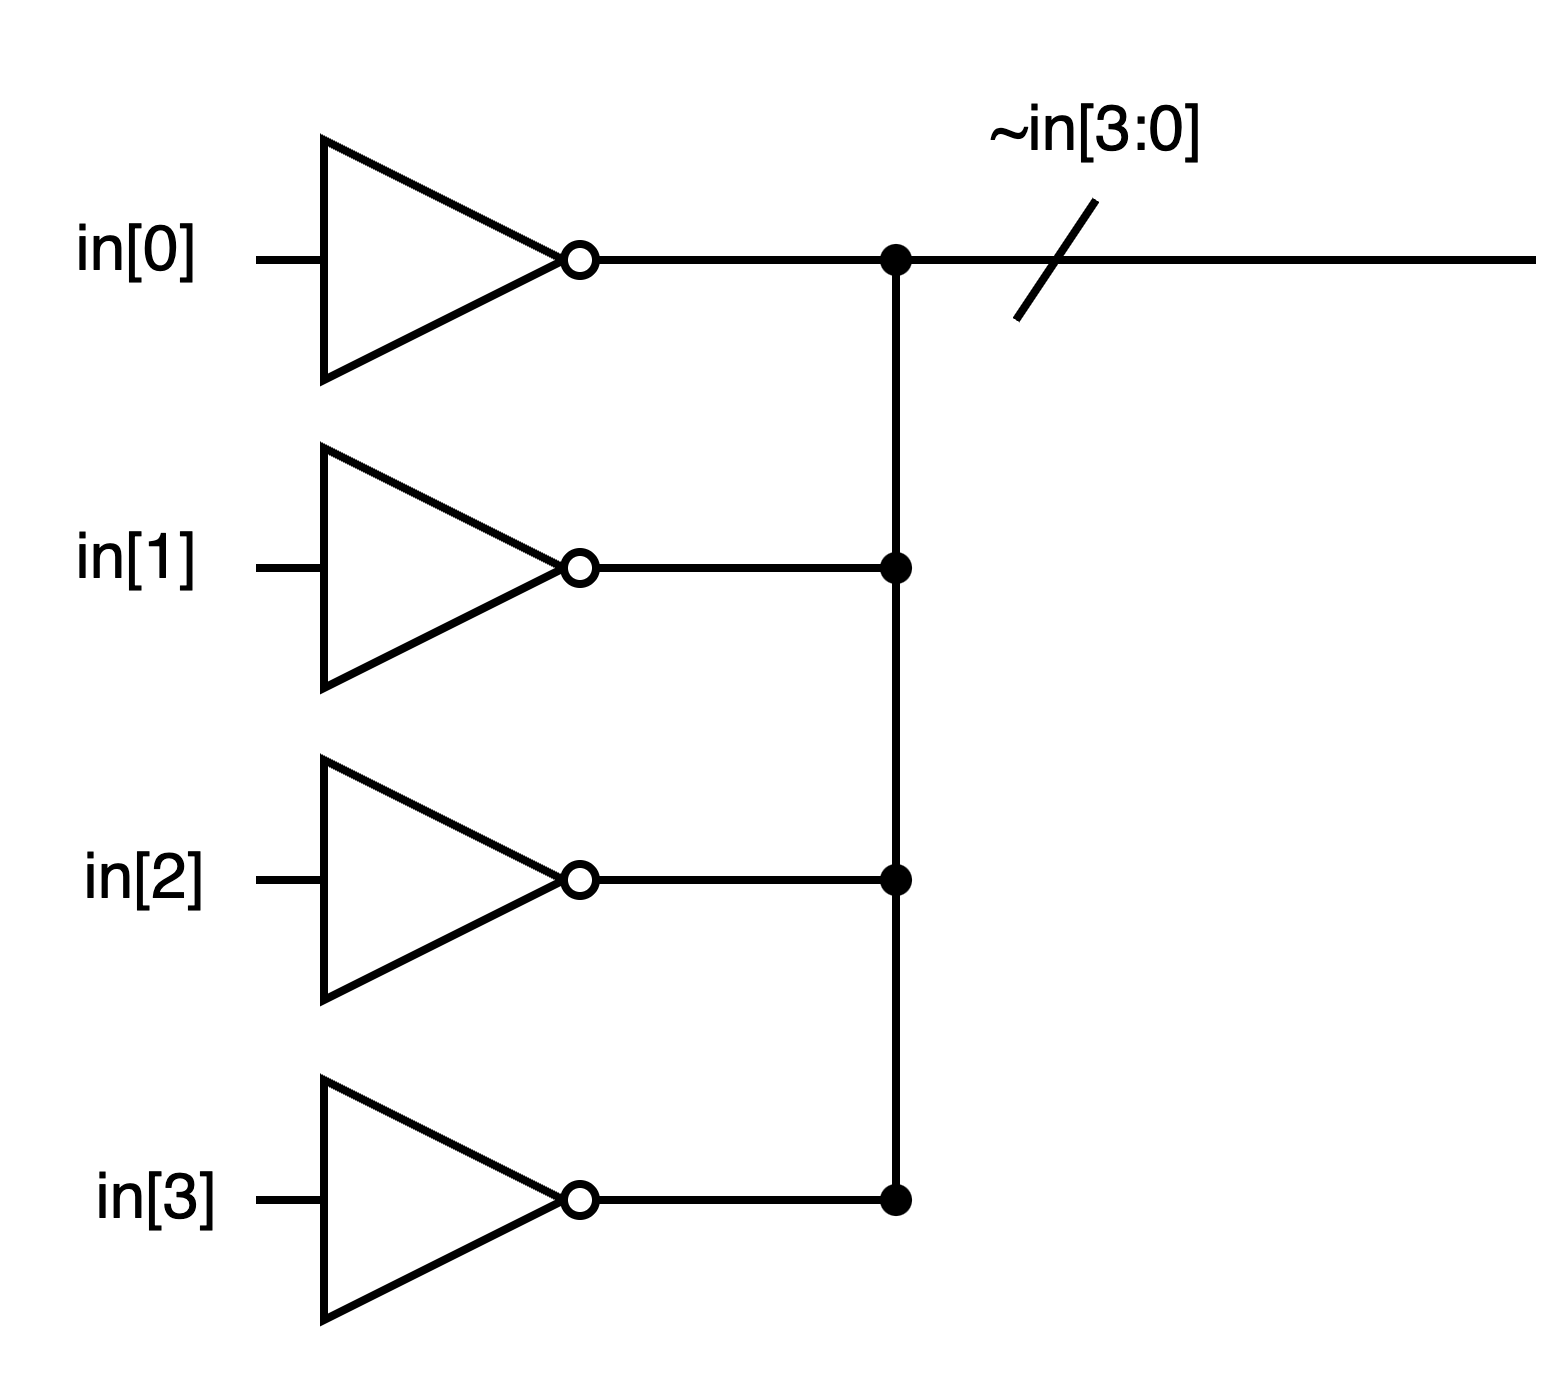
\includegraphics[width=0.3\textwidth]{inverter.png}
  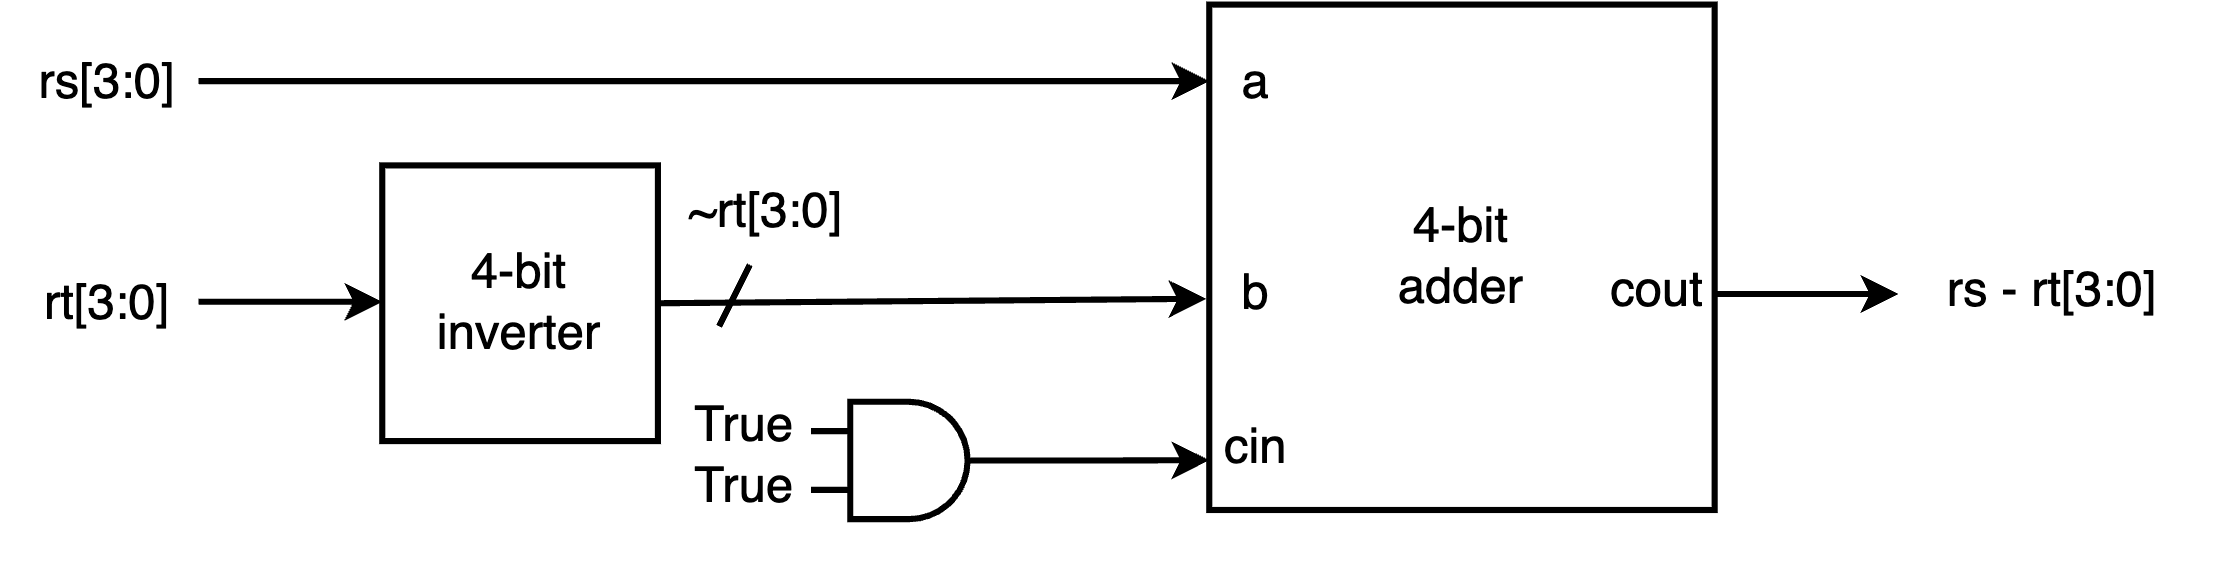
\includegraphics[width=0.6\textwidth]{SUB.png}
  \caption{4-bit Inverter \& SUB Circuit}
  \label{fig:SUB}

\end{figure}
% \newpage
\subsubsection*{ADD}
ADD 的實現同樣基於章節\ref{sec:Q1}實現的加法器,將 $(a, b, cin)$ 設為 $rs, rt, 0$,便是 ADD 的實現\
,如圖 \ref{fig:ADD}。

\begin{figure}[htp]
  \centering
  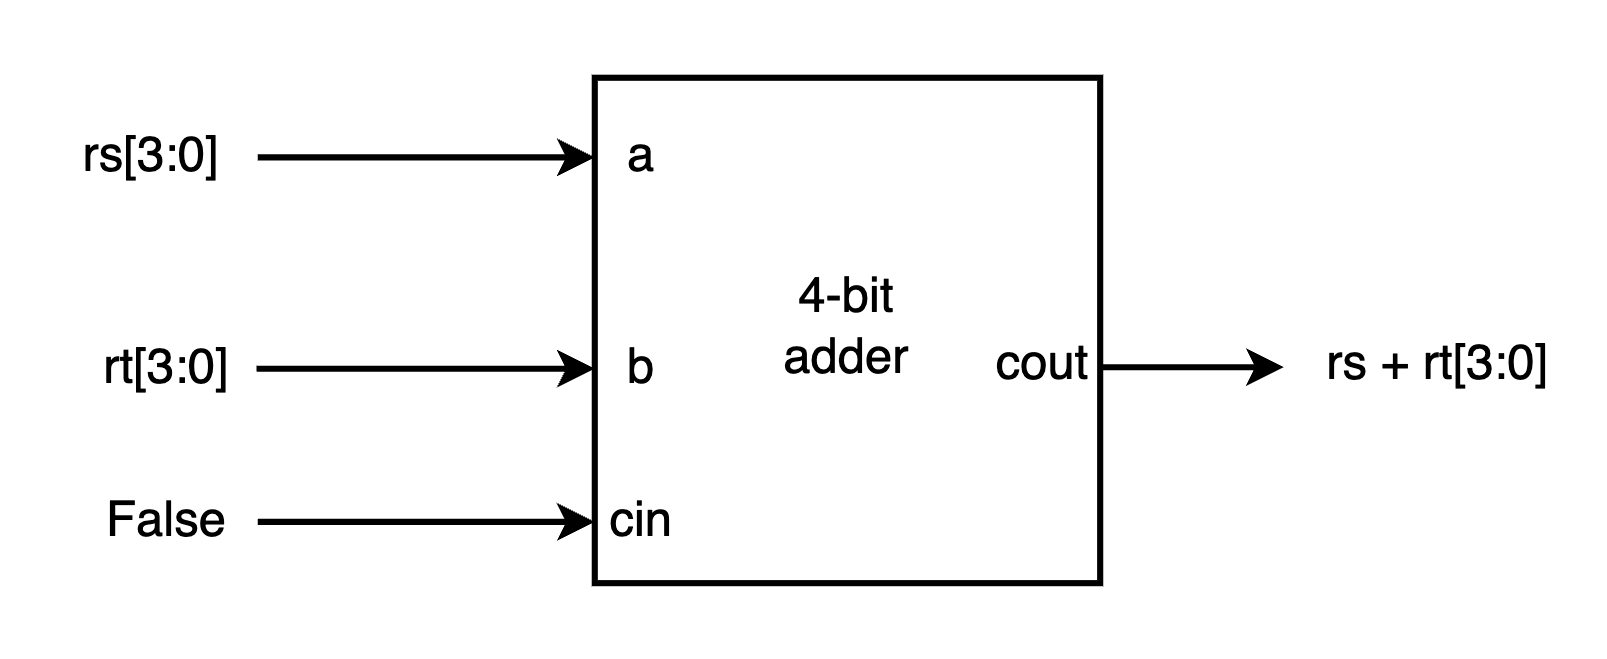
\includegraphics[width=0.4\textwidth]{ADD.png}
  \caption{ADD Circuit}
  \label{fig:ADD}
\end{figure}

\newpage

\subsubsection*{BITWISE OR, BITWISE AND}
如圖 \ref{fig:OR-AND}。

\begin{figure}[htp]
  \centering
  
\includegraphics[width=0.3\textwidth]{BITOR.png}
  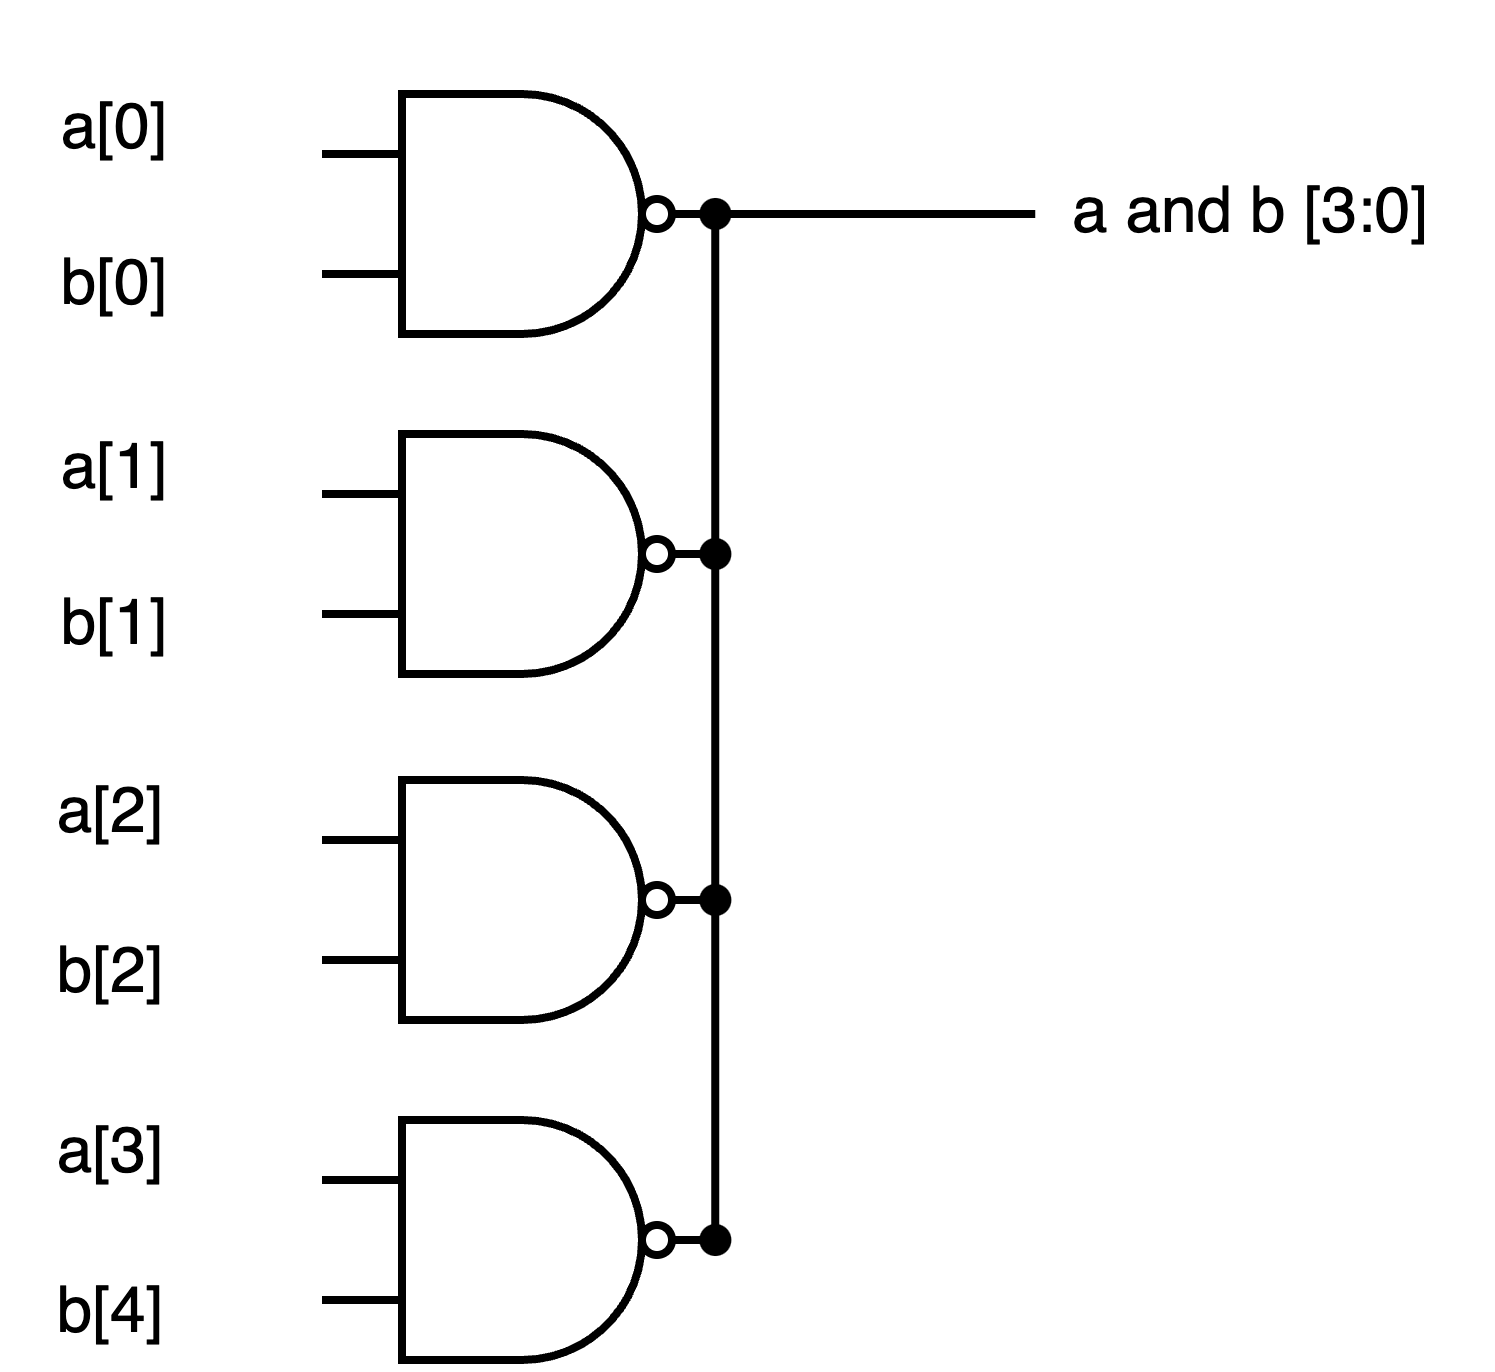
\includegraphics[width=0.3\textwidth]{BITAND.png}
  \caption{Bitwise OR (left), AND (right) Circuit}
  \label{fig:OR-AND}
\end{figure}

\subsubsection*{ARI RIGHT SHIFT}
由於一個 4-bit 的數字以 ARI 的方式右移一位後,$out_0 \sim out_3$ 分別會對應到 $in_1, in_2, in_3, in_3$ \
因此只需要透過與 $1$ 做 AND 能夠實現 assign 的特性,將輸出對應到正確的輸入即可\
如圖 \ref{fig:SHIFT} 右側。


\subsubsection*{CIR LEFT SHIFT}
左移實作方式與右移相同,唯一的區別在於在 CIR 左移的方式,$out_0 \sim out_3$ 分別對應到的是 $in_3, in_0, in_1, in_2$\
如圖 \ref{fig:SHIFT} 左側。


\begin{figure}[htp]
  \centering
  
\includegraphics[width=0.3\textwidth]{LSHIFT.png}
  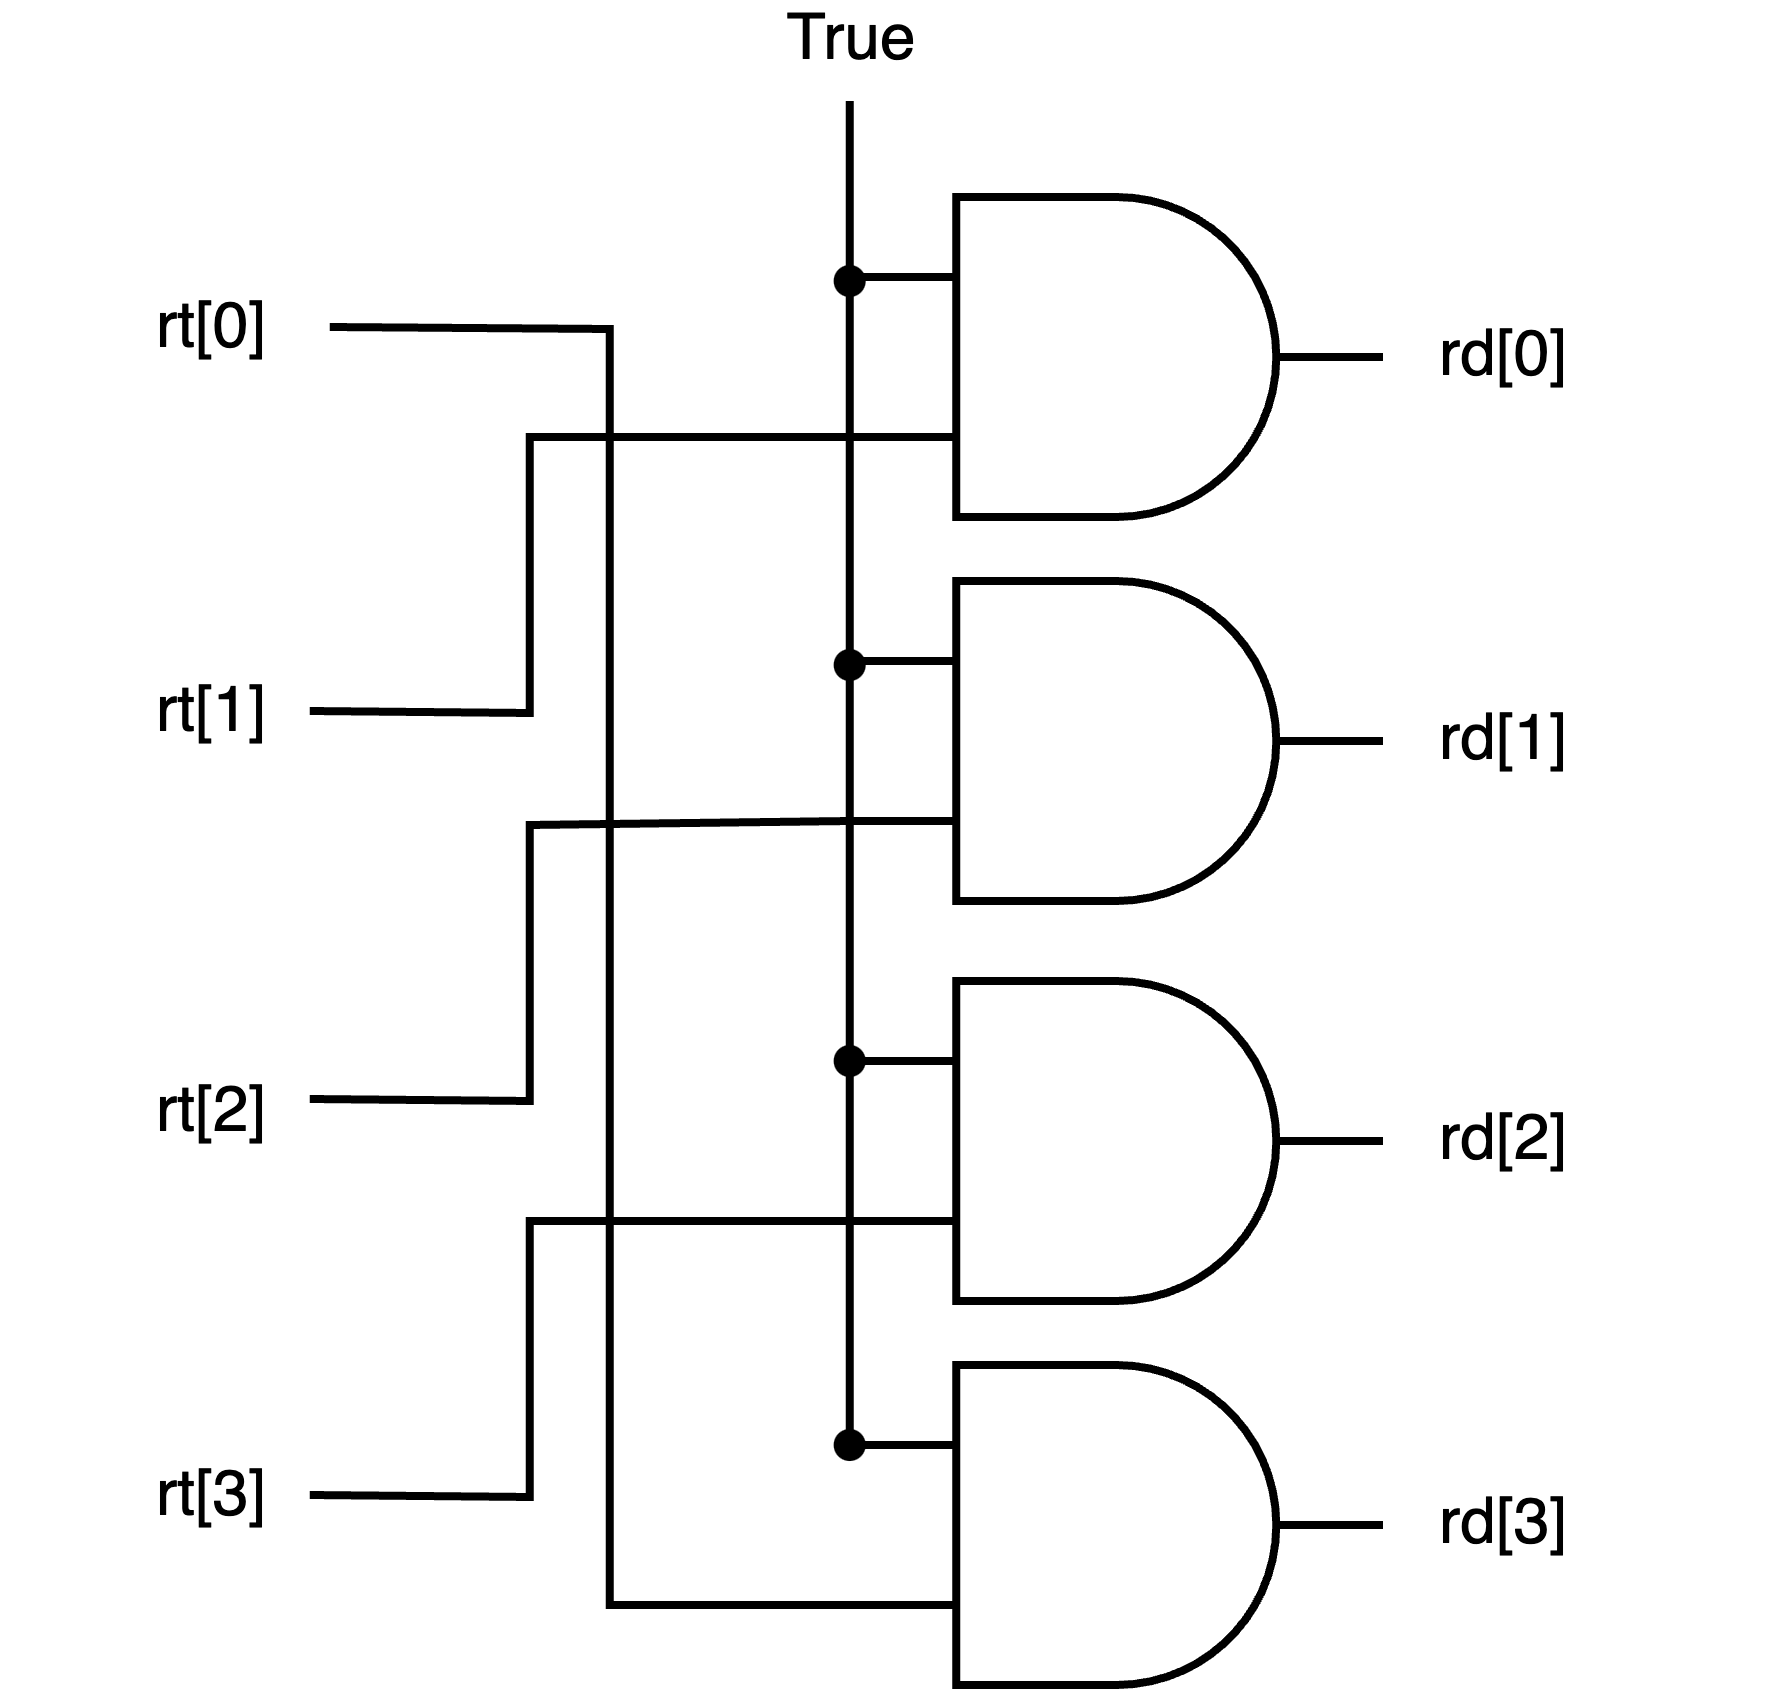
\includegraphics[width=0.35\textwidth]{RSHIFT.png}
  \caption{Left / Right Shift Circuit}
  \label{fig:SHIFT}
\end{figure}

\subsubsection*{COMPARE EQ}
兩個 bit 要相等只有兩種可能:$0, 0$ 或是 $1, 1$,因此 $a = b$ 可以利用 $(!a \& !b) \mid (a \& b)$ 來表示。\ 
如果我們要判斷兩個 4-bit 數字是否一樣,只需分別對四個位元做以上操作,並確認是否都為 True,即可,\
如圖 \ref{fig:EQ} 所示。最終加上的 $1110_{(2)}$ 為題目要求。

\begin{figure}[htp]
  \centering
  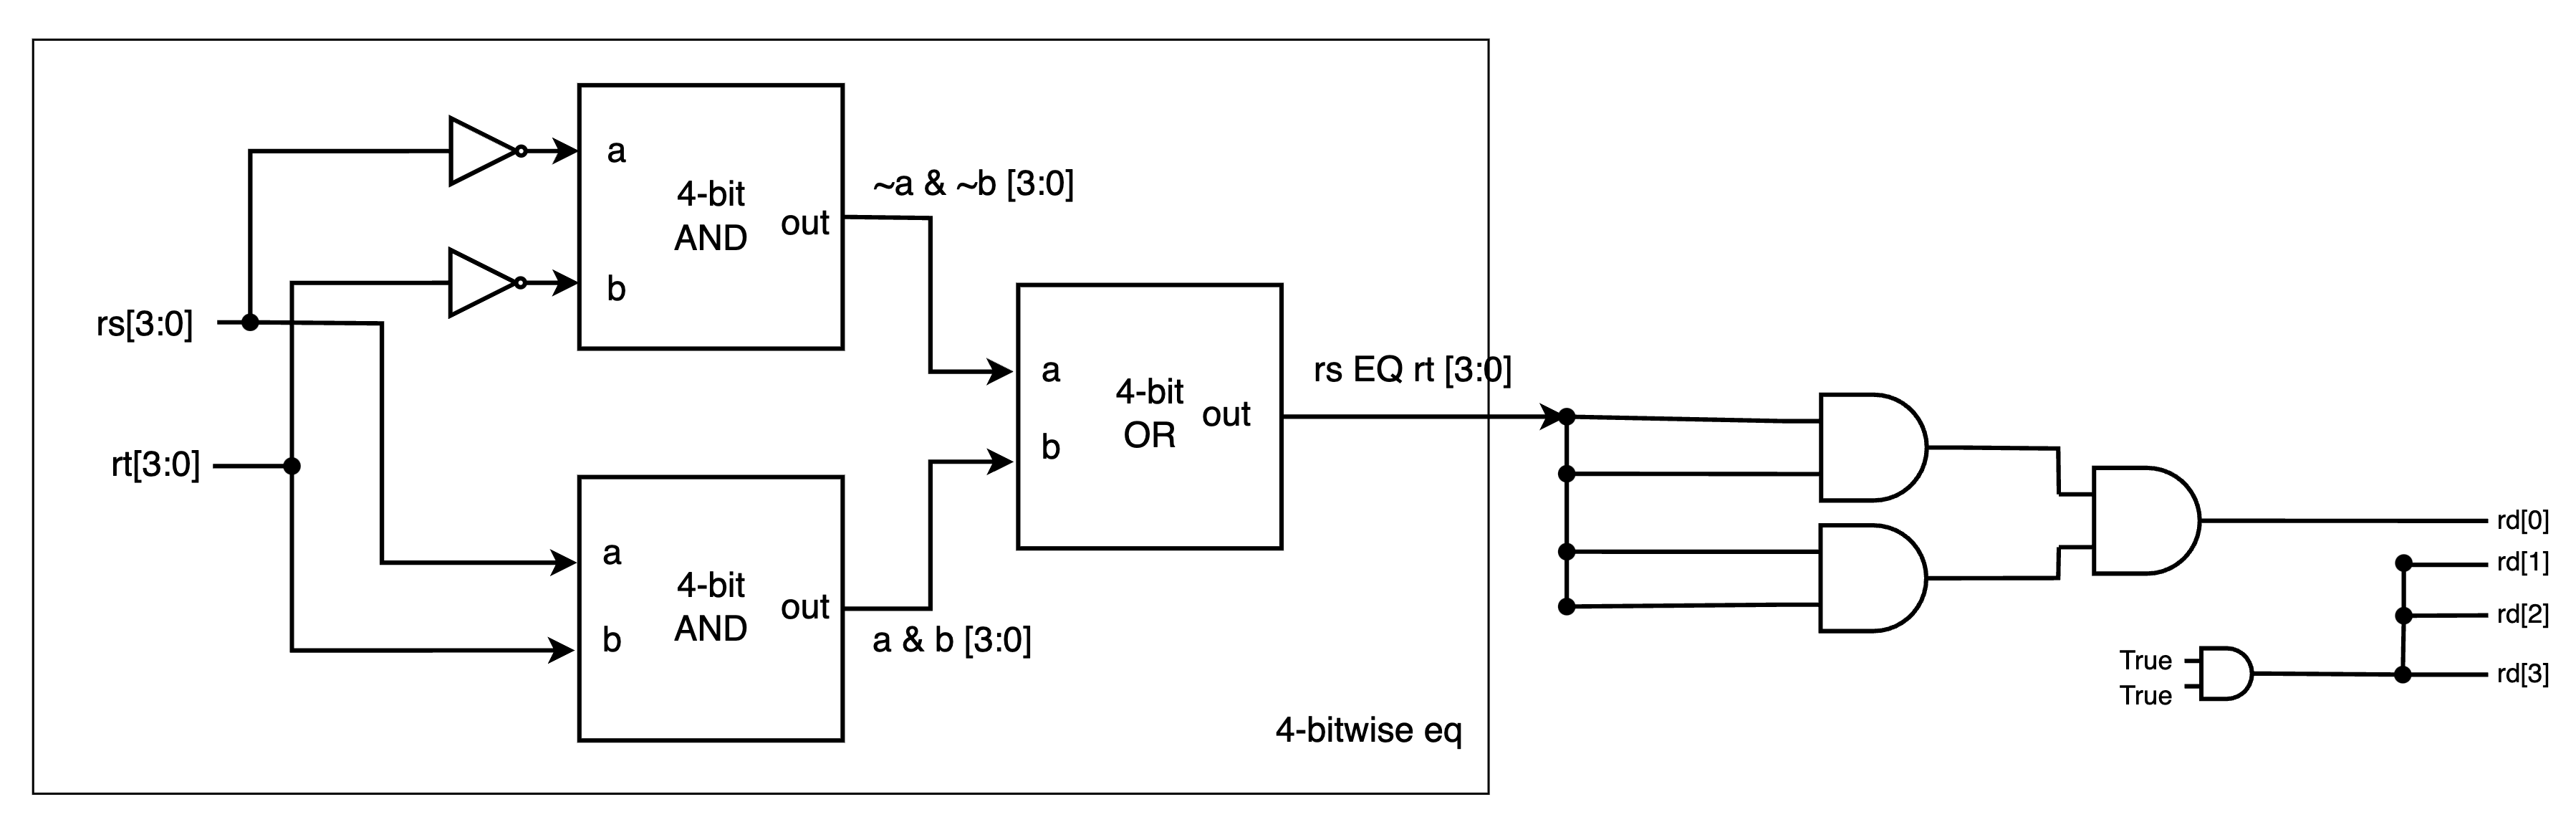
\includegraphics[width=\textwidth]{EQ.png}
  \caption{Compare EQ Circuit}
  \label{fig:EQ}
\end{figure}

\newpage

\subsubsection*{COMPARE LT}
由於比較的結果決定於由高位數來第一個不同的位元,因此一個 4-bit 的比較小於將基於以下步驟:
\begin{enumerate}
  \item 比較 $rs[3]$ 是否 $< rt[3]$
  \item 若上個步驟為 False 且 $rs[3] = rt[3]$,則比較 $rs[2]$ 是否 $< rt[2]$
  \item 重複上述步驟,直到找到第一個不同的位元
\end{enumerate}

這幾個步驟可以寫成一個表達式:
$out = (rs[3] < rt[3]) \mid (rs[3] = rt[3] \& rs[2] < rt[2]) \mid (rs[3] = rt[3] \& \
rs[2] = rt[2] \& rs[1] < rt[1]) \mid (rs[3] = rt[3] \& rs[2] = rt[2] \& rs[1] = rt[1] \& rs[0] < rt[0])$

根據以上式子實作便可得到比較的結果,最後再加上題目規定的 $1010_{(2)}$ 即可。

\begin{figure}[htp]
  \centering
  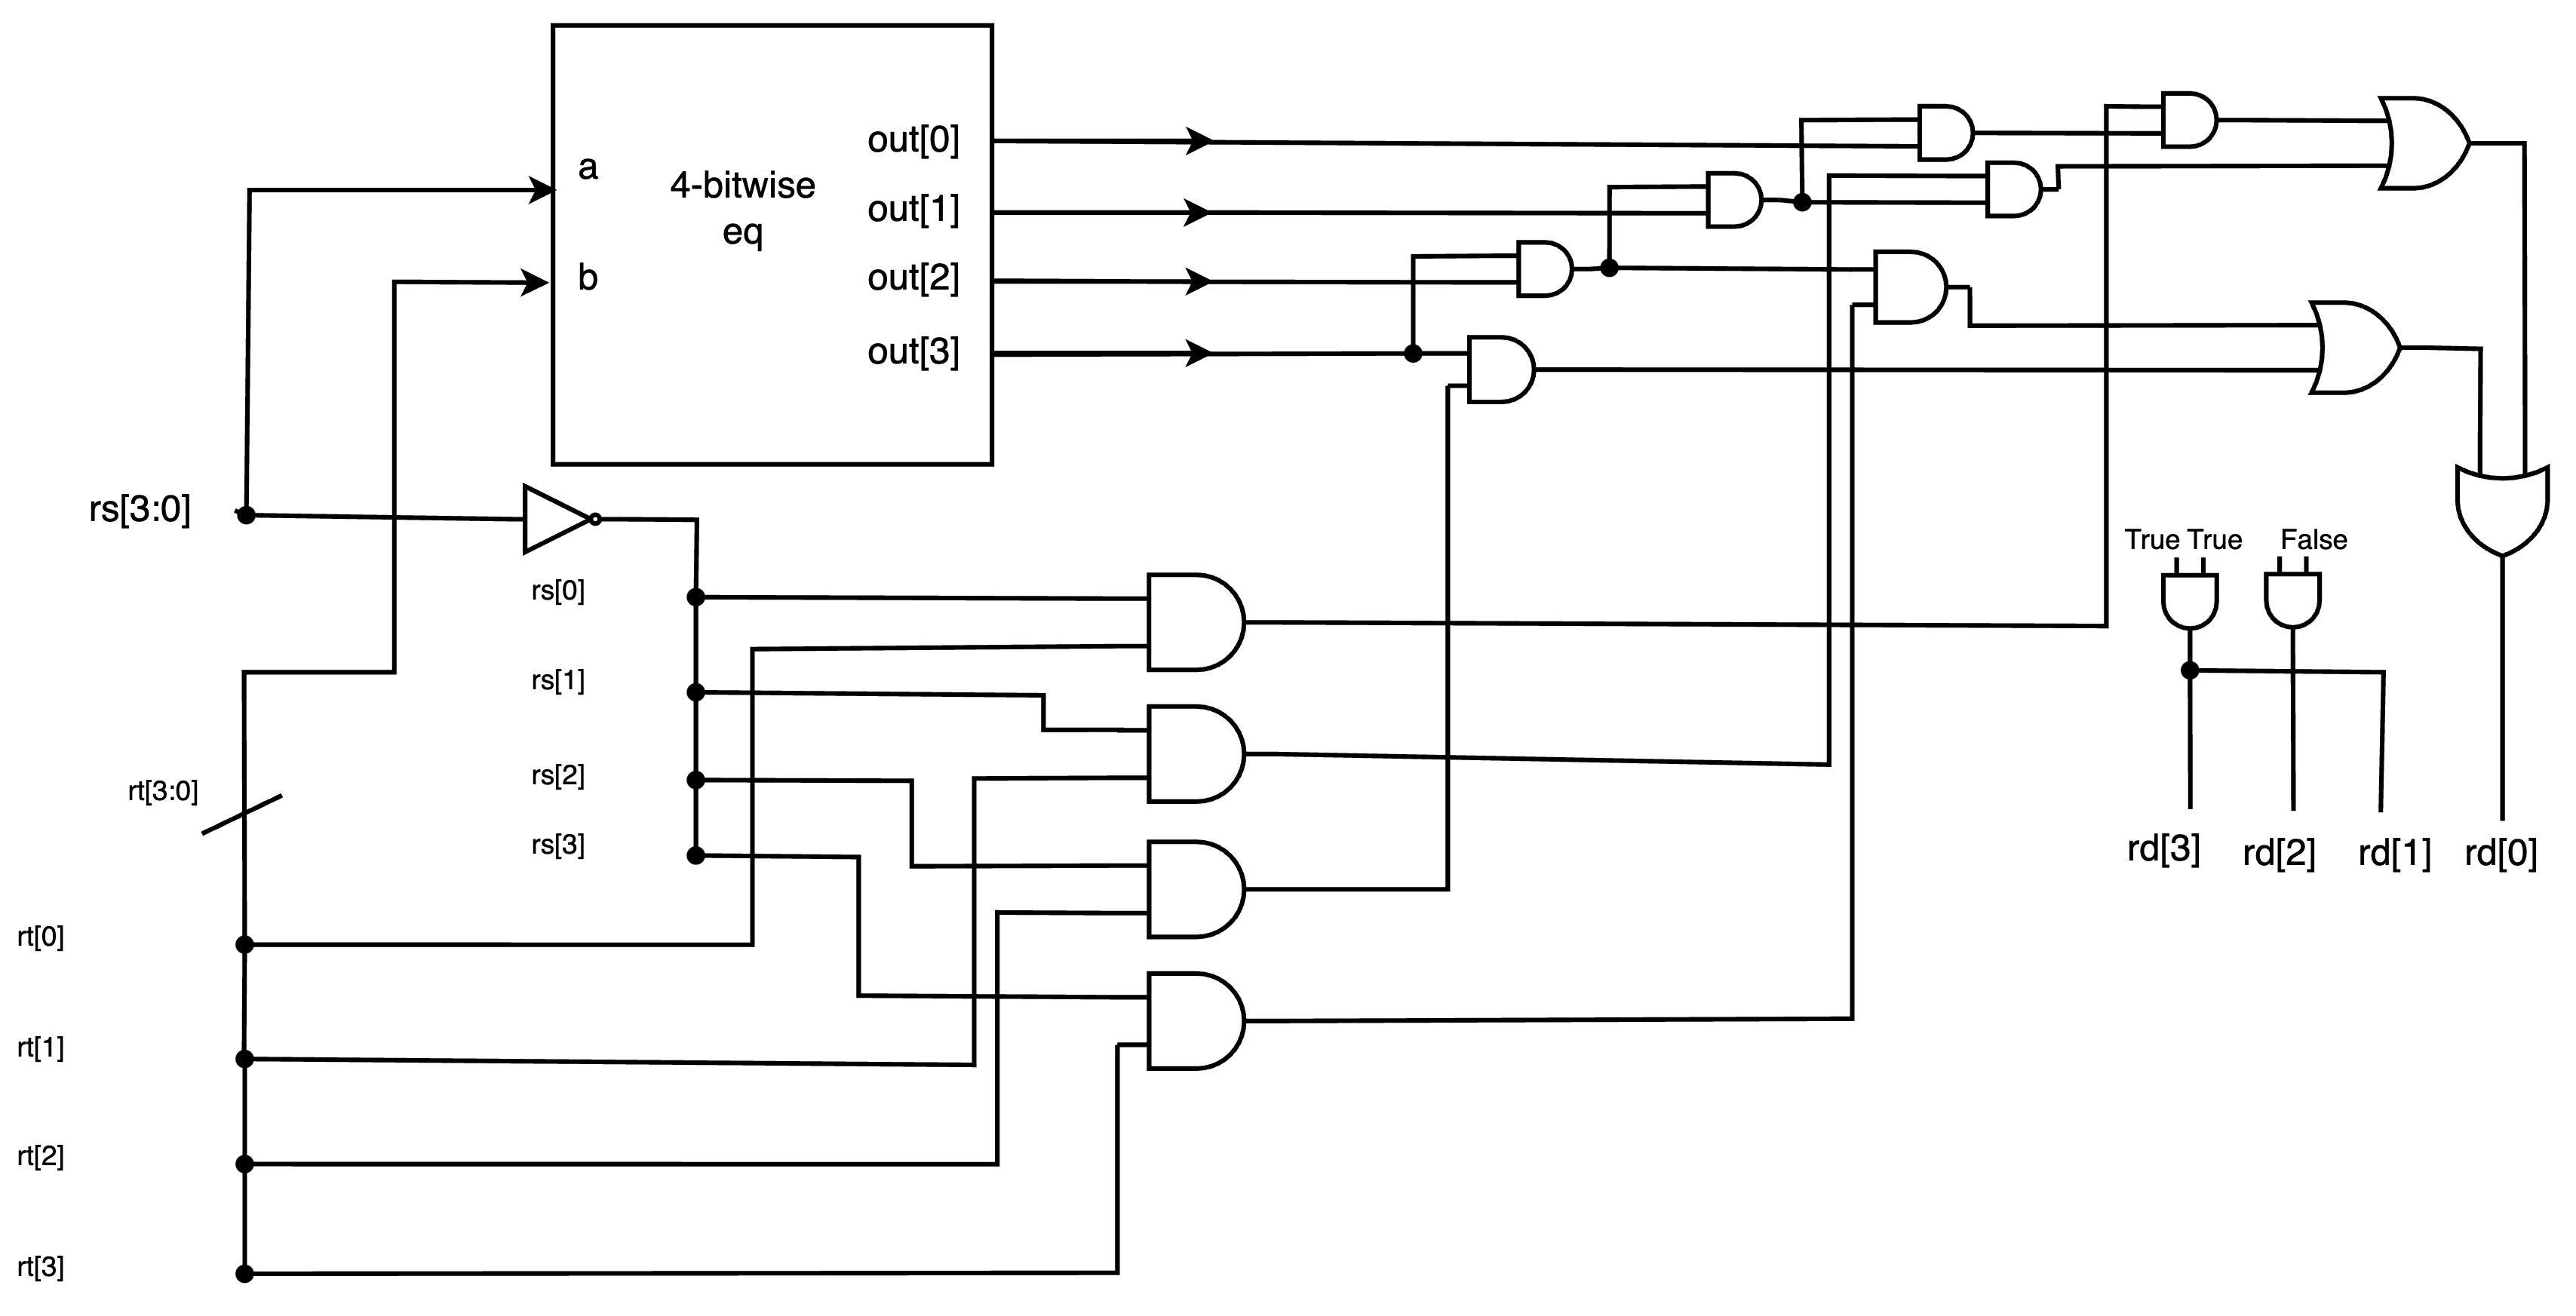
\includegraphics[width=\textwidth]{LT.png}
  \caption{Compare LT Circuit}
  \label{fig:LT}
\end{figure}

\subsection{Decoder}
首先將 Executor 生成的結果依 $OP\_Code$ 轉成十進位後表示的值導至線路 $0 \sim 7$(例如當 $OP\_Code = 000_{(2)}$,導向線路 0,$OP\_Code = 101$ 時導向線路 5),由於指令只有八種,\
因此我們可以使用七個 2-to-1 mux,並分成三個階段來實現 Decoder:

\begin{enumerate}
  \item 第一階段,將 $sel[0]$ 作為 MUX 的 select bit,並依照 $OP\_Code$ 轉成十進位後的值(可參考先前的圖 \ref{fig:Q2-spec}) \
  分成 $(0, 1), (2, 3), (4, 5), (6, 7)$,各自輸入到一個 MUX 中,當 $sel[0] = 0$ 時選擇前者,反之選擇後者,便可將八種指令篩選成四種,\
  這裡以 $01, 23, 45, 67$ 來表示四個組別。
  \item 第二階段,與第一階段相同的規則,將四個組別兩兩一組:$(01, 23), (45, 67)$ 將 $sel[1]$ 作為 MUX 的 select bit,便可以將四種指令再篩選成兩種:$0123, 4567$。
  \item 第三階段,也是一樣的規則,將 $sel[2]$ 作為 MUX 的 select bit,便可以得到我們所需要的輸出。
\end{enumerate}

\begin{figure}[htp]
  \centering
  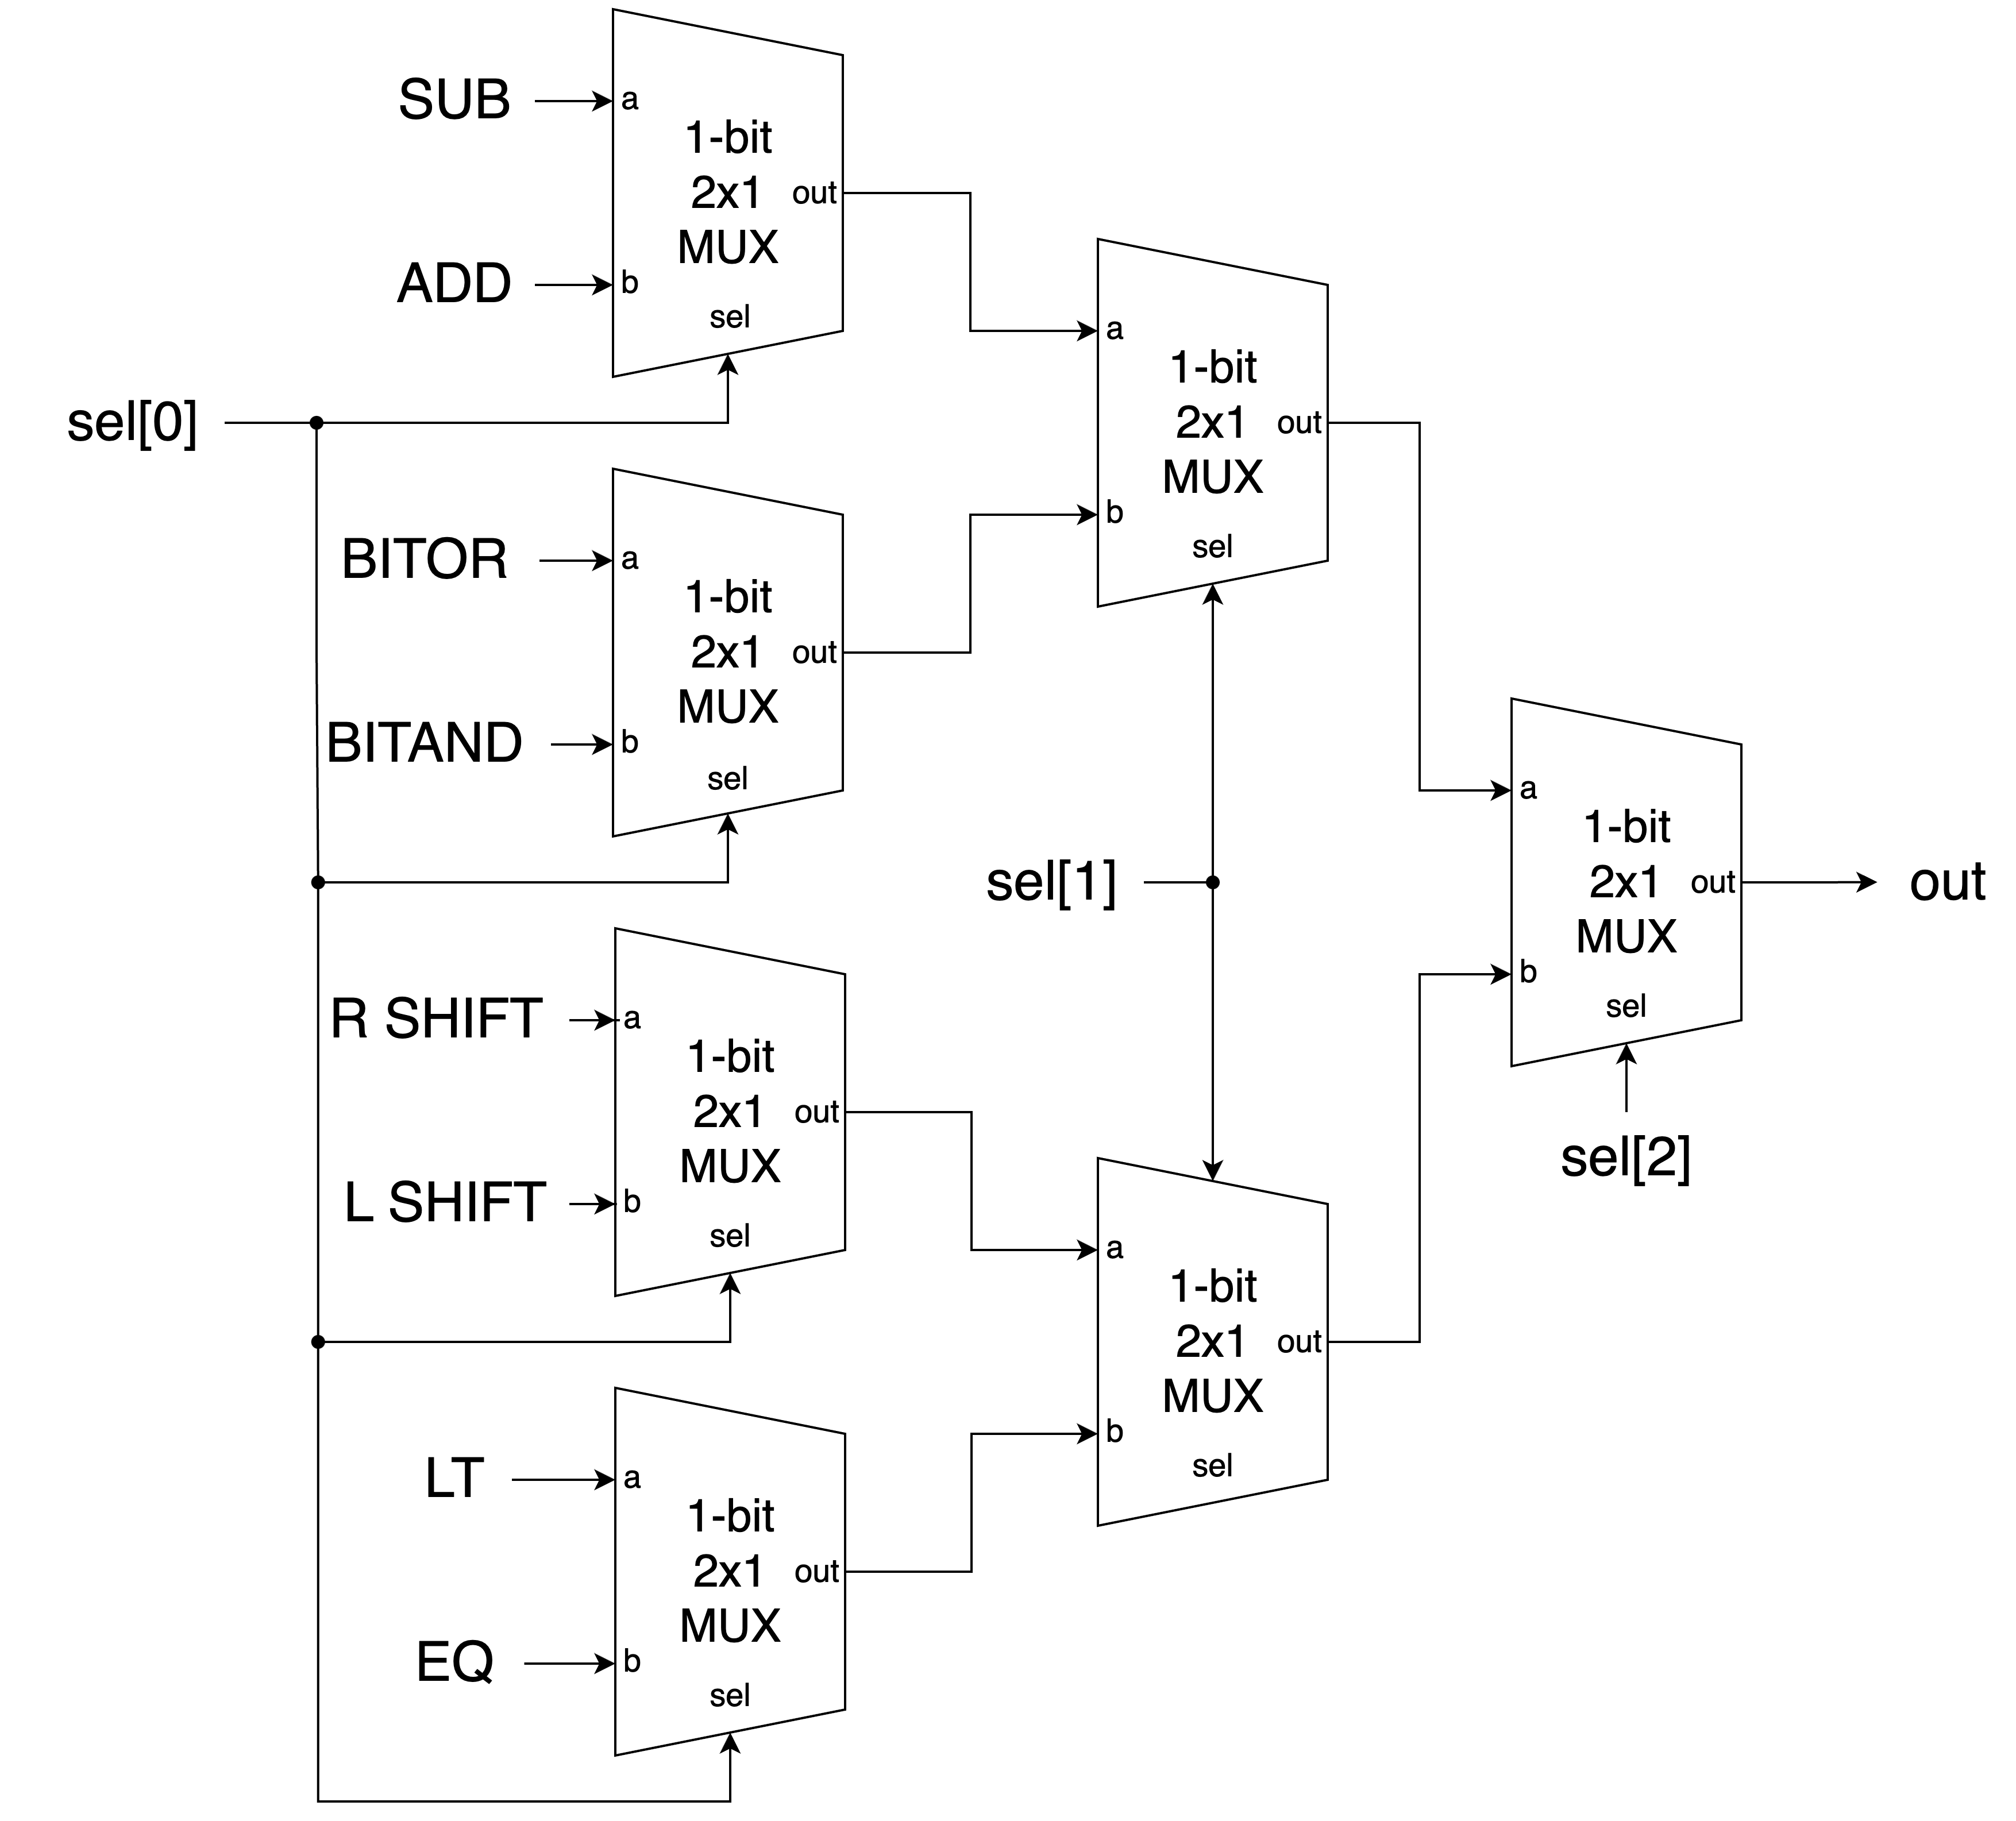
\includegraphics[width=0.9\textwidth]{Q2-decoder.png}
  \caption{Decoder Circuit}
  \label{fig:Decoder}
\end{figure}

\newpage

\subsection{Testbench}

$rs, rt$ 都是 4-bit,$OP\_Code$ 則是 3-bit,因此總共枚舉了 $2^{11} = 2048$ 種可能。
\par
由於次數過多,因此同樣採用 if statement 的方式,並搭配 verilog 的 case 語法實現判斷是哪一種操作,並分成兩個部分進行操作:

\begin{figure}[ht]
  \centering
  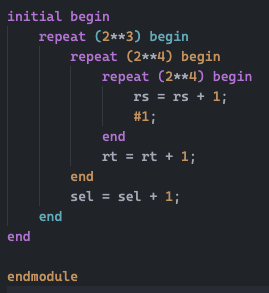
\includegraphics[width=0.3\textwidth]{Q2-tb1.png}
  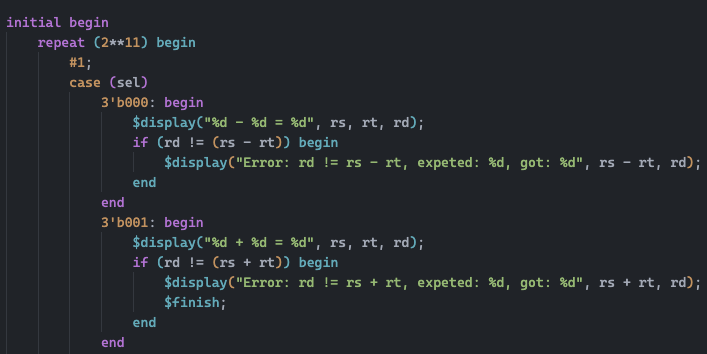
\includegraphics[width=0.653\textwidth]{Q2-tb2.png}
  \caption{Q2 testbench code}
  \label{fig:Q2_tb}
\end{figure}

第一部分用來枚舉所有可能,第二部分則是負責判斷是否有錯誤。

\begin{figure}[!ht]
  \centering
  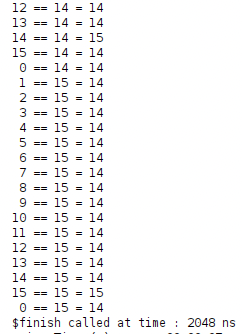
\includegraphics[width=0.15\textwidth]{Q2-display.png}
  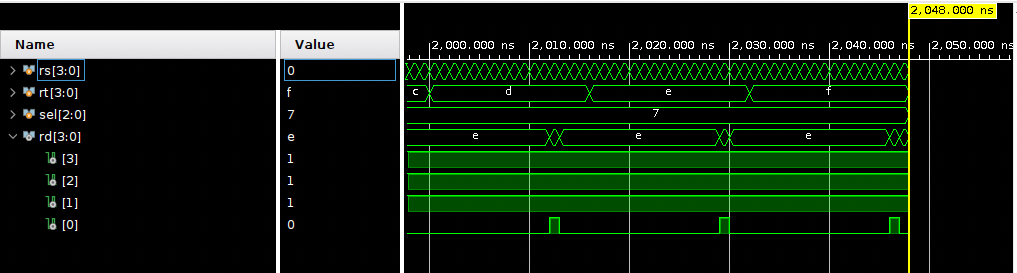
\includegraphics[width=0.8\textwidth]{Q2-wave.png}
  \caption{Q2 testbench results,有跑完 2048 次模擬代表沒有錯誤}
  \label{fig:Q2_display}
\end{figure}

\newpage

\section{Q3: 8-bit carry-lookahead adder}
\label{sec:Q3}

一般的加法器,由於需要等待上一個 Full Adder 輸出進位值,因此在運算時間會隨著處理的位元數線性增加,\
運算階段的複雜度可以說是 $\mathcal{O}(n)$,如果我們可以提前算出每個 Full Adder 的 $cin$ 值,\
那麼運算階段的複雜度就可以降到 $\mathcal{O}(1)$,而這也是 Carry Lookahead Adder 的核心概念。

CLA 的運算過程如下圖(\ref{fig:CLA-3step}),可以分為:PG Generator, CLA Generator, Adder 三個部分:

\begin{figure}[htp]
  \centering
  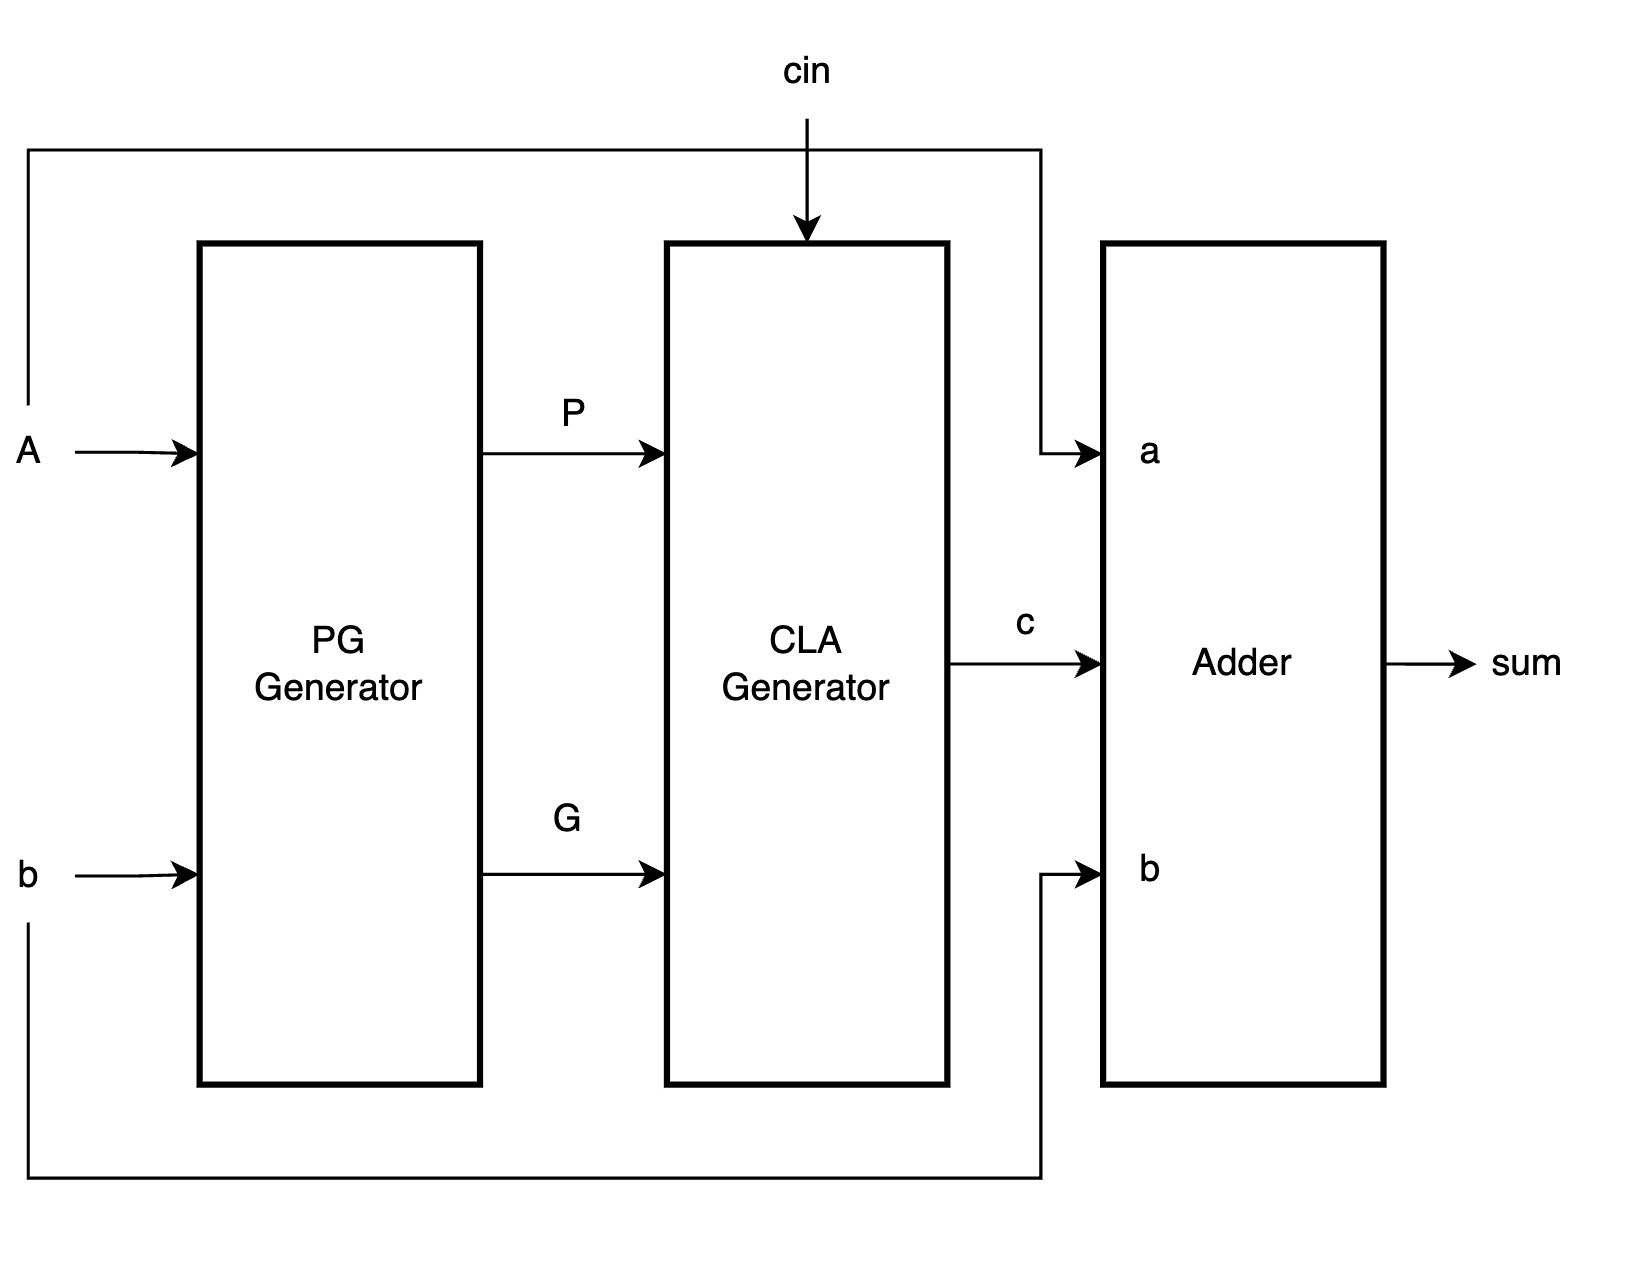
\includegraphics[width=0.5\textwidth]{CLA-3step.png}
  \caption{CLA 3-step}
  \label{fig:CLA-3step}
\end{figure}

\subsection{PG Generator}
首先定義 $P, G$:
\begin{itemize}
  \item $G$: Generate,但表是否產生進位,用 $a \& b$ 實現
  \item $P$: Propagate,代表是否會傳遞收到的進位,可以用 $a \^{} b$ 或是 $a \mid b$ 實現(因為實際上只需要判斷 $(0, 1)$ 的情況\
            如果是 $(1, 1)$ 的話那麼該位的 $G$ 就會是 True,便用不到 $P$ 了)
\end{itemize}

實現方式如圖 \ref{fig:PG_Gen},\
這步驟生成完 $P, G$ 後,就會將其傳遞到下一步的 CLA Generator。

\begin{figure}[htp]
  \centering
  
\includegraphics[width=0.3\textwidth]{PG_Gen.png}
  \caption{PG Generator Circuit}
  \label{fig:PG_Gen}
\end{figure}

\newpage

\subsection{CLA Generator}

\subsubsection*{4-bit CLA Generator}
此步驟的目標是為了生成出 $C_i$,我們可以列出這個式子:
$$C_i = G_{i - 1} + P_{i - 1} \cdot C_{i - 1}$$

可以發現,這個式子中,$C_i$ 依舊對 $C_{i - 1}$ 具有依賴性,這並不符合我們希望加速的目標,因此我們可以嘗試將 $C_{i - 1}$ 展開:
\begin{align*}
  C_i &= G_{i - 1} + P_{i - 1} \cdot C_{i - 1} \\
      &= G_{i - 1} + P_{i - 1} \cdot (G_{i - 2} + P_{i - 2} \cdot C_{i - 2}) \\
      &= G_{i - 1} + P_{i - 1} \cdot G_{i - 2} + P_{i - 1} \cdot P_{i - 2} \cdot C_{i - 2} \\
      &= \ \ \ \ \ \ \ \ \ \ \ \ \ \ \ \ \ \ \ \ \ \ \ \ \ \ \ \ \ \ \ \ \ \ \vdots
\end{align*}

在 4-bit Generator (不計算 $c_4$)的情況下,展開後的則為:
\begin{align*}
  & C_1 = G_0 + P_0 \cdot C_0 \\
  & C_2 = G_1 + P_1 \cdot C_1 \\
  &= G_1 + P_1 \cdot (G_0 + \underline{(P_0 \cdot C_0)}) \\
  & = (G_1 + (P_1 \cdot G_0)) + (P_1 \cdot \underline{(P_0 \cdot C_0)}) \\
  & C_3 = G_2 + (P_2 \cdot C_2) \\
  & = G_2 + (P_2 \cdot (G_1 + (P_1 \cdot G_0) + \underline{(P_1 \cdot (P_0 \cdot C_0))}) \\
  & = G_2 + (P_2 \cdot G_1) + (P_2 \cdot (P_1 \cdot G_0)) + ((P_2 \cdot P_1) \cdot \underline{(P_0 \cdot C_0)}) \
\end{align*}
\label{math: CLA_Generator}

其中,底線的部分代表重複計算的值,我們可以直接將其重複利用,以降低 Gate 的面積與效能。\ 
並且將 AND 部分平行計算,並將能夠兩兩分組的部分,以分治的概念來合併,便能將所需的運算次數降低到 $\log n$ 次。

利用以上辦法,我們就能夠實現 4-bit 的 CLA Generator。

\begin{figure}[htp]
  \centering
  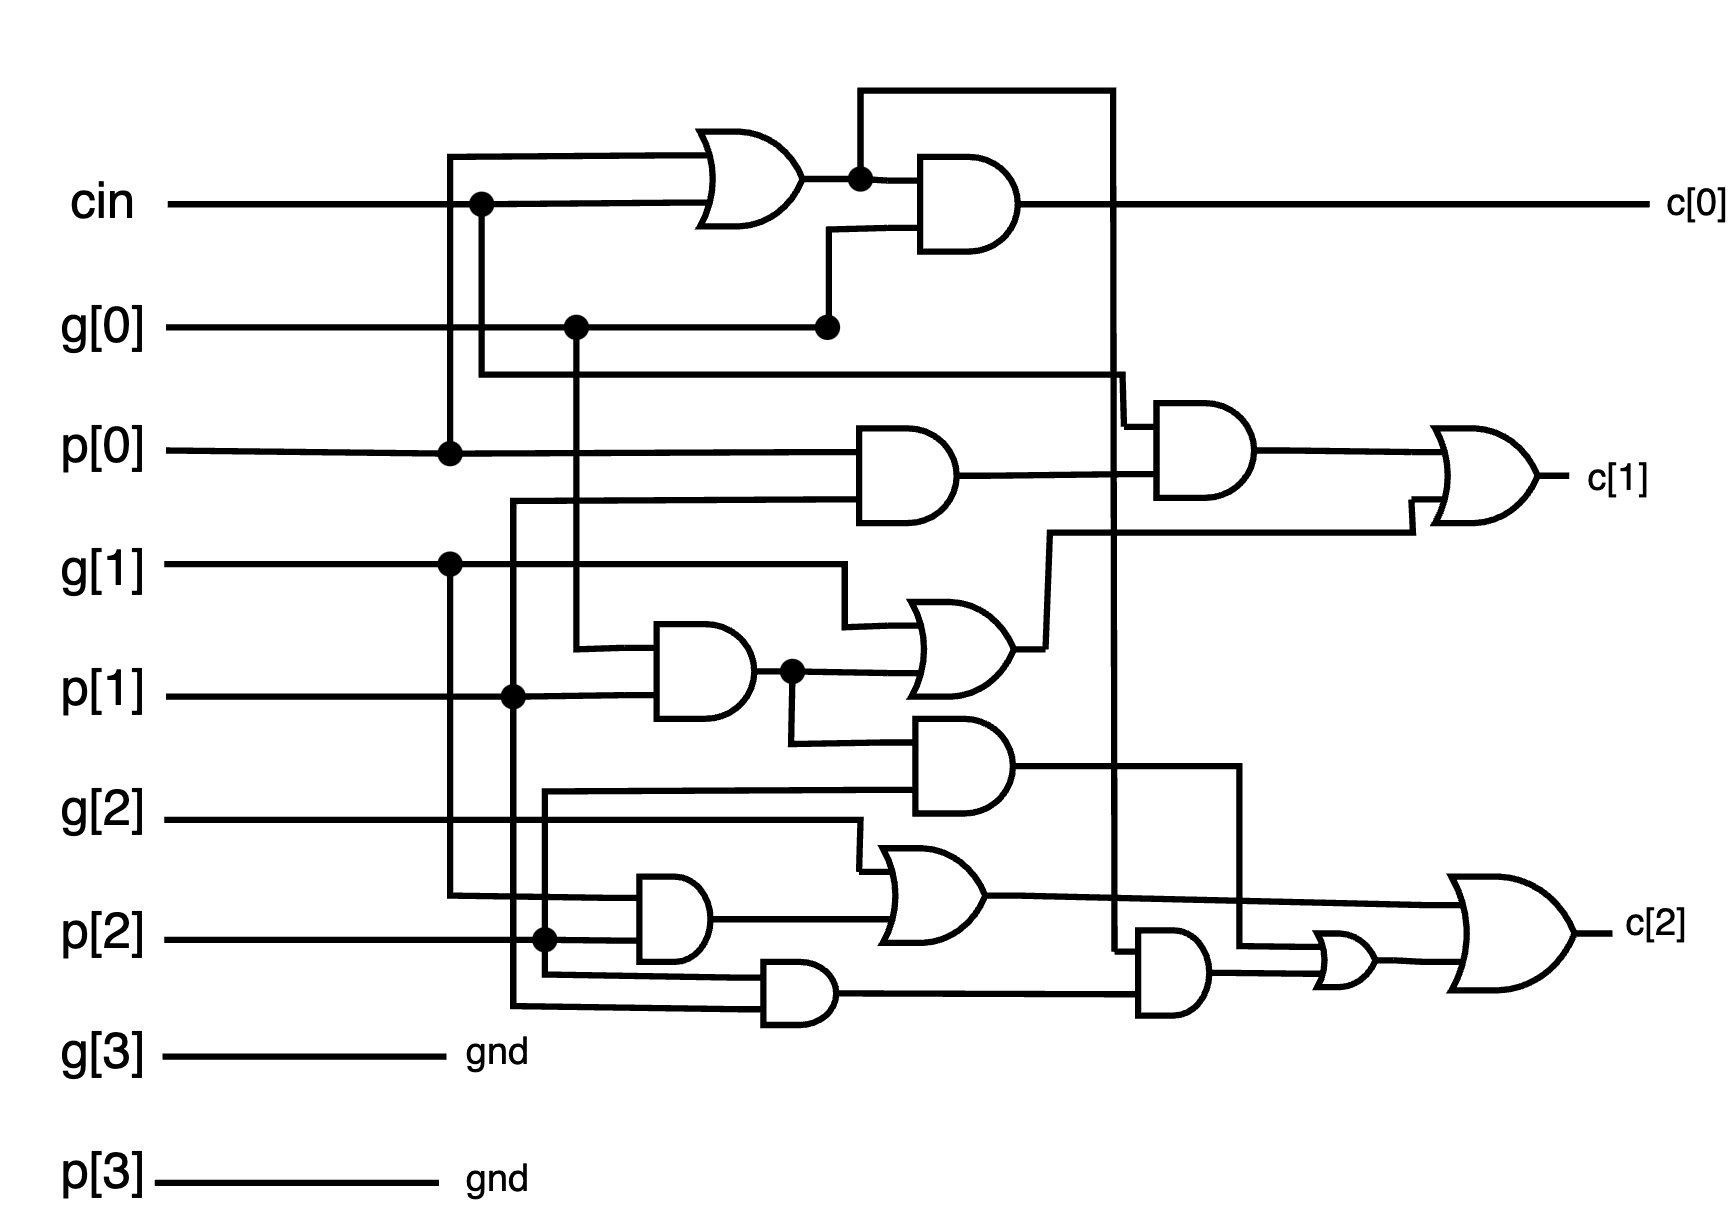
\includegraphics[width=0.6\textwidth]{4-bit-Gen.png}
  \caption{4-bit CLA Generator Circuit}
  \label{fig:4-bit-Gen}
\end{figure}

\newpage

\subsubsection*{2-bit CLA Generator}
這個部分需要接收兩組 $p[3:0], g[3:0], p[7:4], g[7:4]$ 並計算出 $c_4, c_8$,根據上一段的推導,\
計算方法為:
\begin{align*}
  & C_4 = G_3 + (P_3 \cdot C_3) \\
  & = G_3 + (P_3 \cdot G_2) + (P_2 \cdot G_1) + (P_2 \cdot (P_1 \cdot G_0)) + ((P_2 \cdot P_1) \cdot \underline{(P_0 \cdot C_0)})) \\
  & = G_3 + \underline{(P_3 \cdot G_2)} + (P_3 \cdot \underline{(P_2 \cdot G_1)}) + ((P_3 \cdot P_2) \cdot \underline{(P_1 \cdot G_0)}) \\
  & \ \ + (P_3 \cdot \underline{((P_2 \cdot P_1) \cdot (P_0 \cdot C_0))})
\end{align*}

但是這樣實在是太冗長了,根據 reference\footnote{https://en.wikipedia.org/wiki/Carry-lookahead\_adder\#Implementation\_details},\
$P, G$ 能夠被轉換為 group propagate (GP) 以及 group generate (GG):
$$GP = P_0 \cdot P_1 \cdot P_2 \cdot P_3$$
$$GG = G_3 + G_2 \cdot P_3 + G_1 \cdot P_3 \cdot P_2 + G_0 \cdot P_3 \cdot P_2 \cdot P_1$$

而 $c_8$ 的計算方式也是同樣的方式,於是我們便完成了 2-bit 的 CLA Generator。

\begin{figure}[htp]
  \centering
  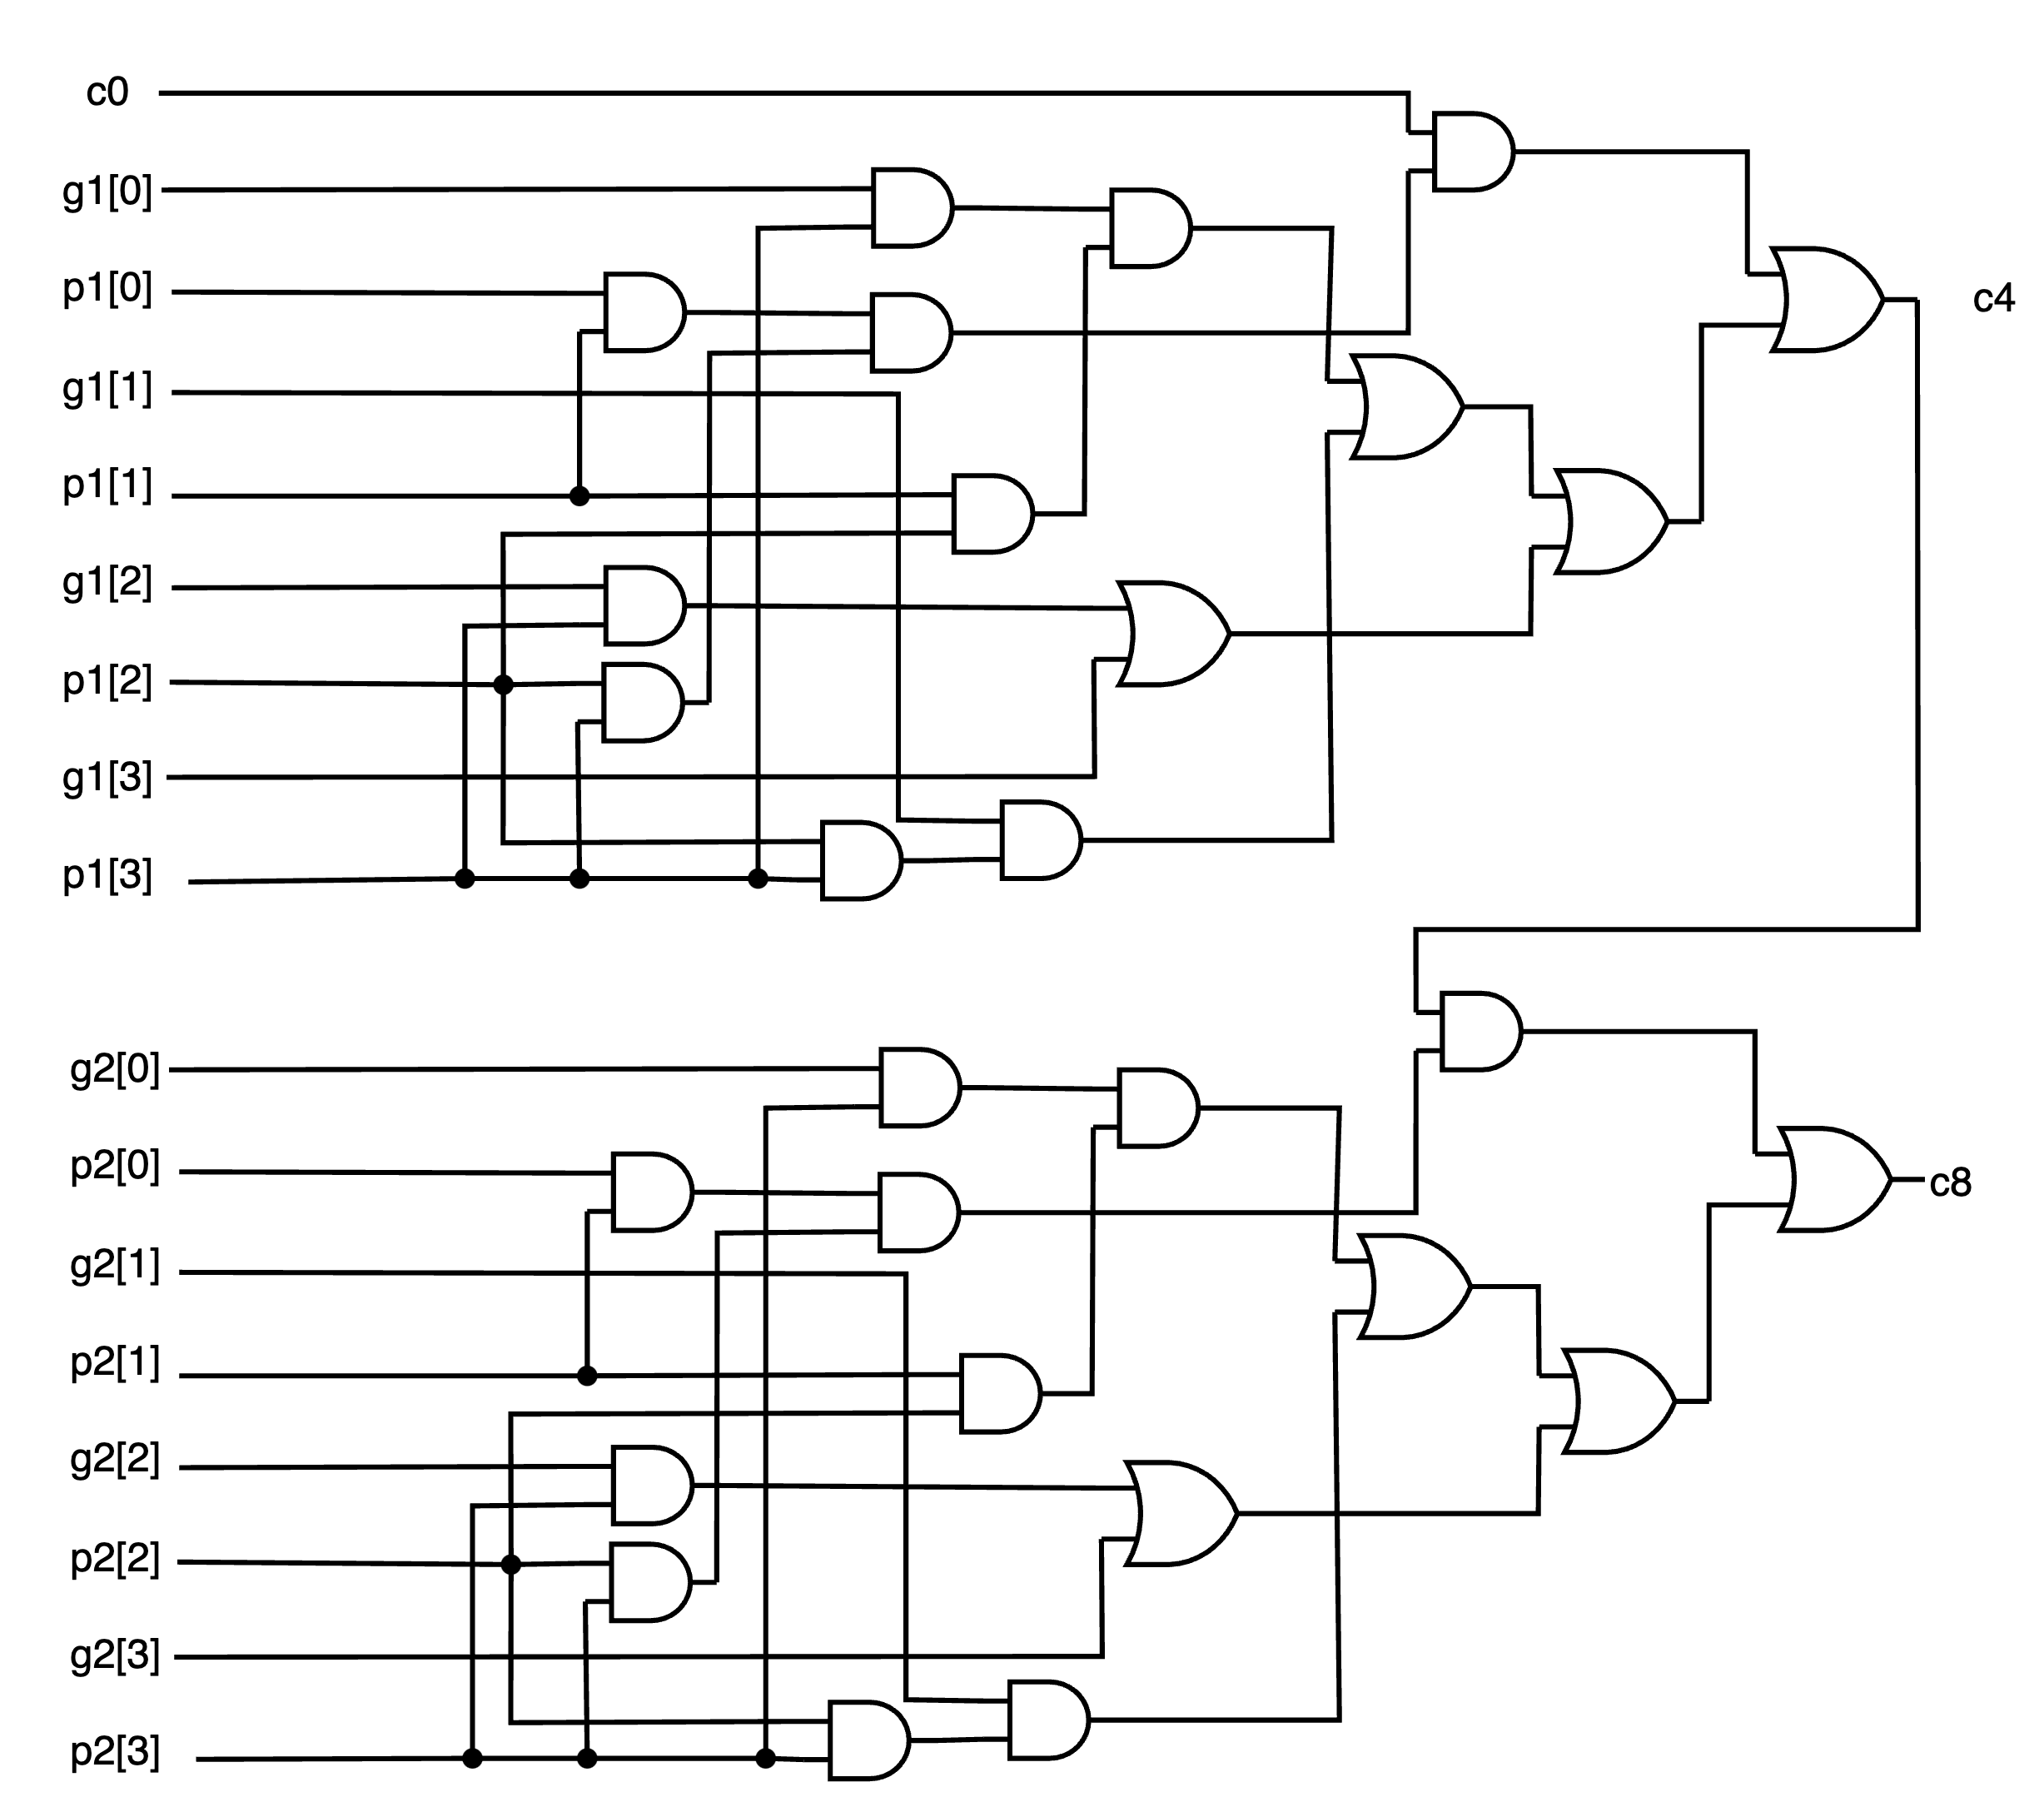
\includegraphics[width=0.7\textwidth]{2-bit-Gen.png}
  \caption{2-bit CLA Generator Circuit}
\end{figure}

\newpage

\subsection{Adder}

建立 $8$ 個沒有 cout 的 Adder(畢竟 carry bit 已經在 Generator 計算出來),並將 $a, b, cin$ 分別接上 $rs, rt$ 以及 CLA Generator 的輸出,即可算出答案。

\begin{figure}[htp]
  \centering
  
\includegraphics[width=0.5\textwidth]{Adder.png}
  \caption{Adder}
\end{figure}

\subsection{Overall}
\begin{figure}[htp]
  \centering
  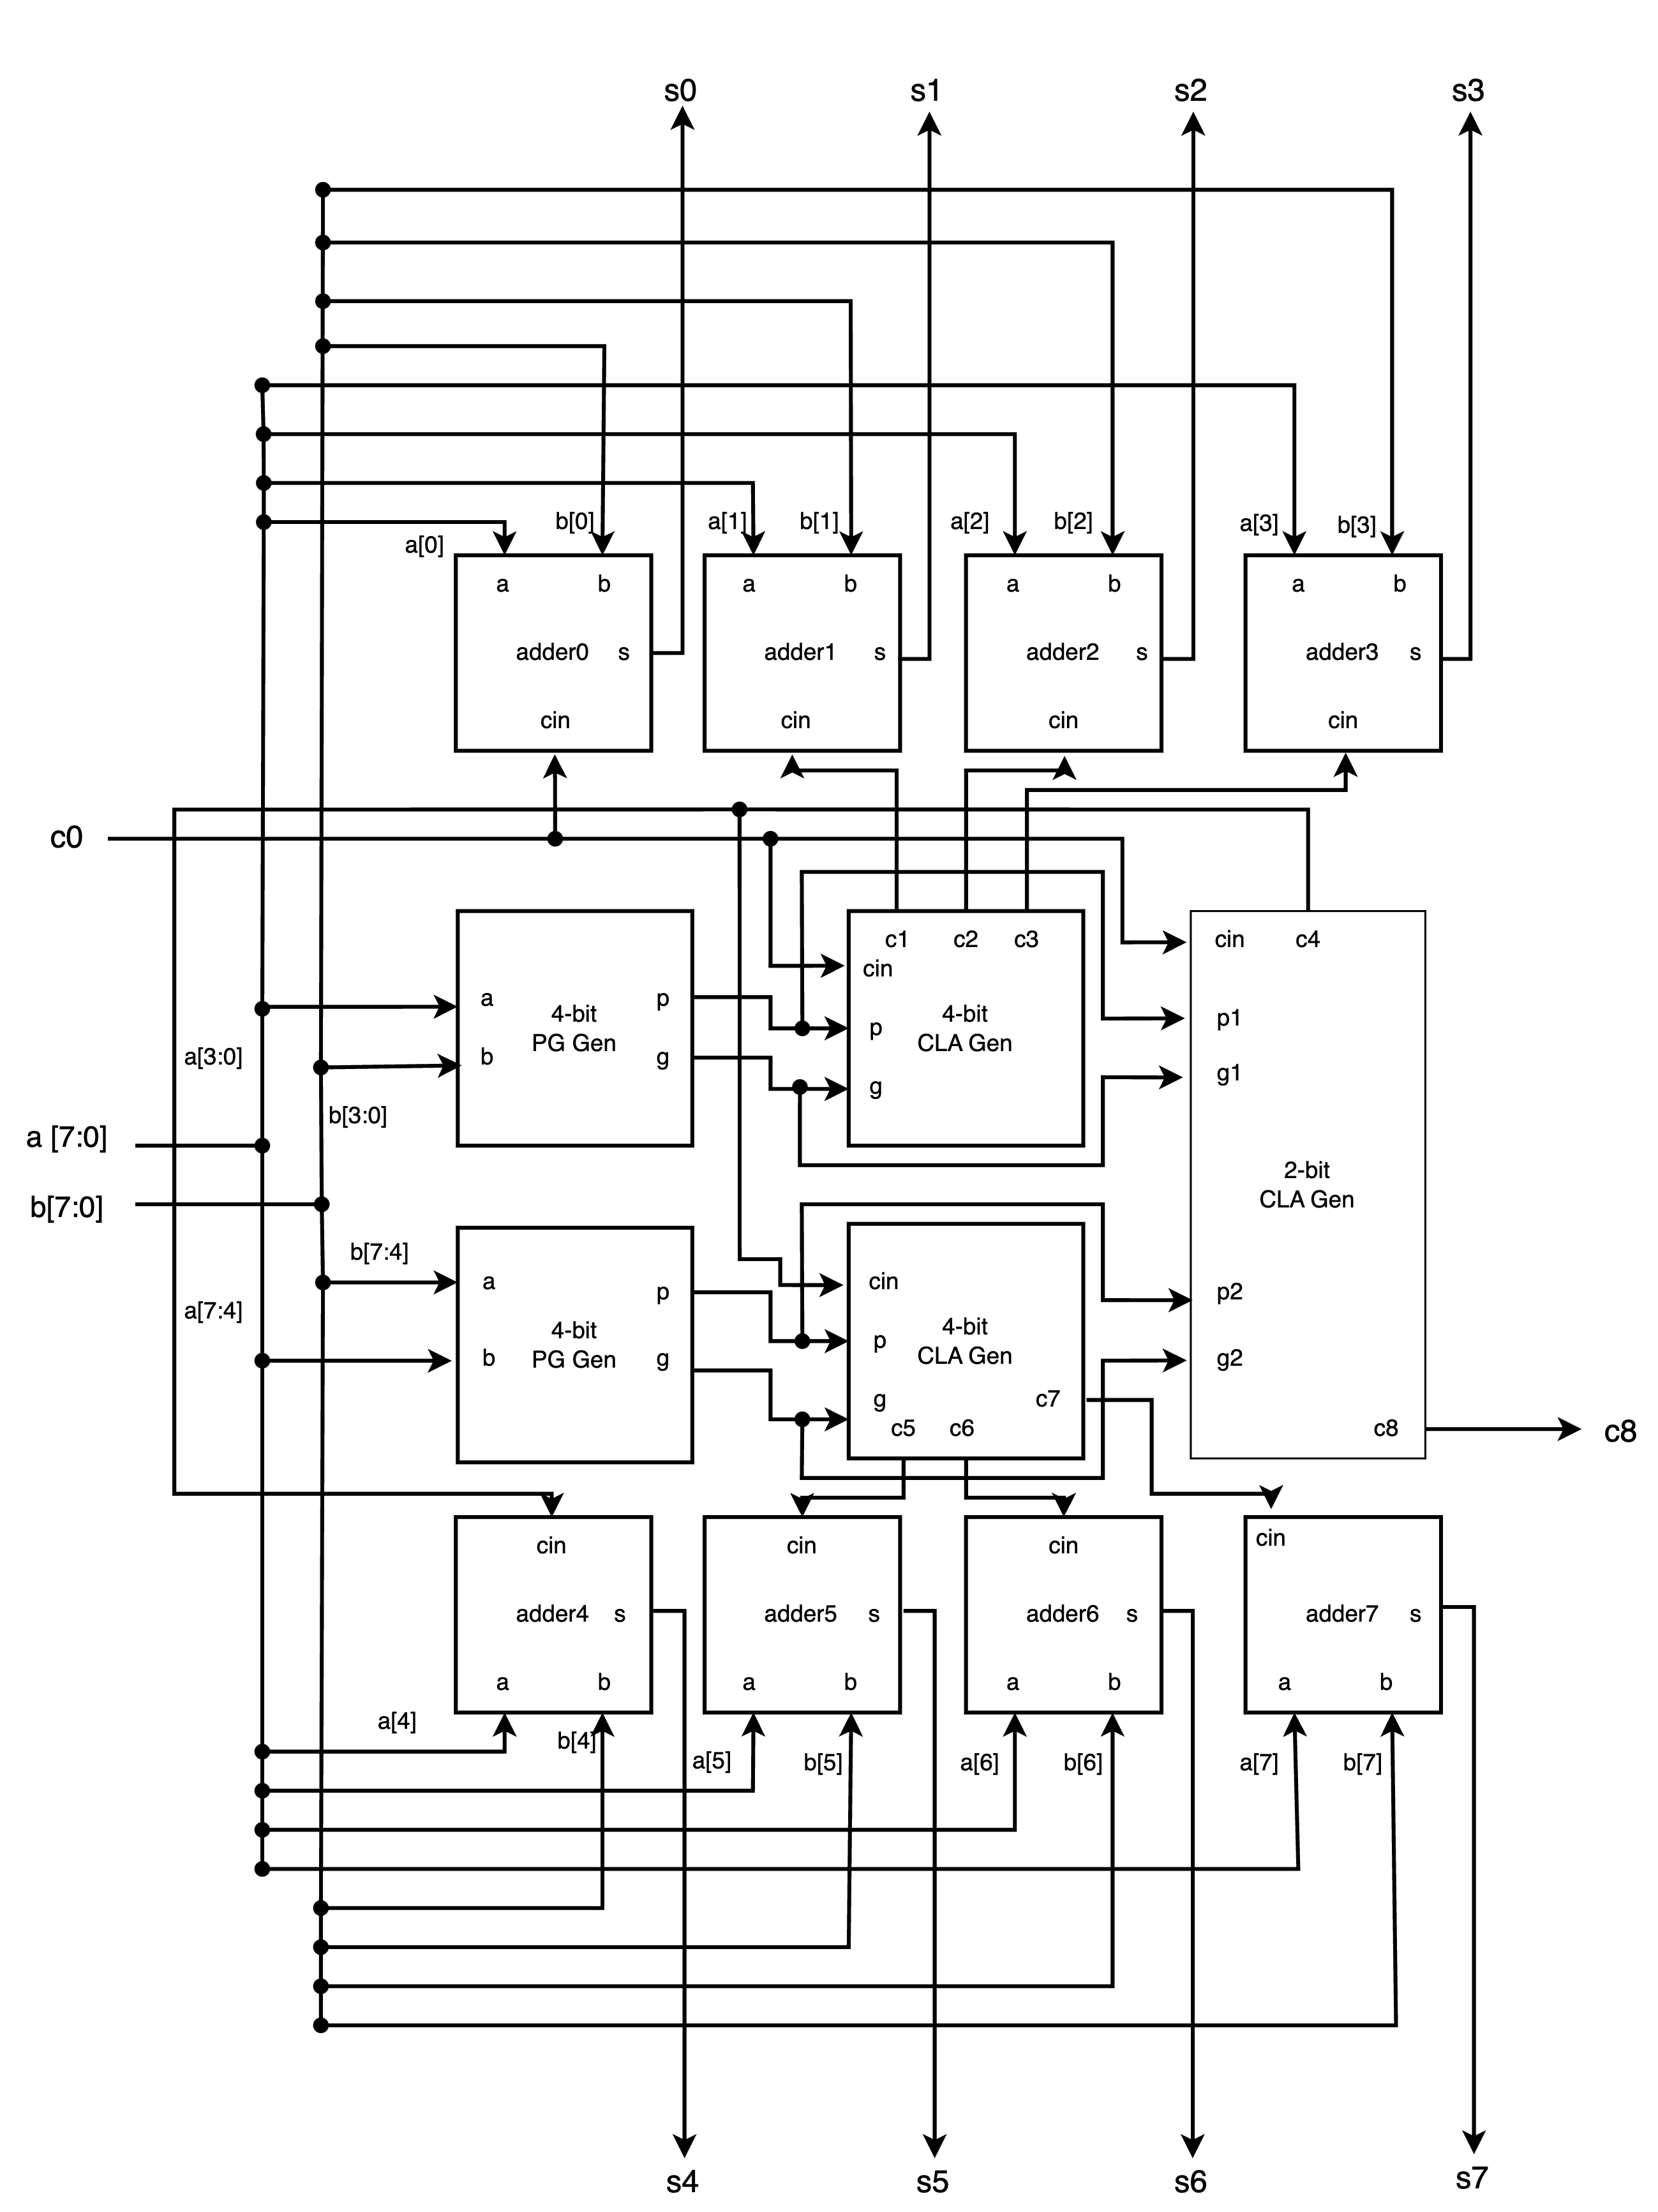
\includegraphics[width=0.9\textwidth]{8-bit_CLA.png}
  \caption{8-bit CLA}
\end{figure}

\newpage

\subsection{Testbench}

如同前面的章節,我們枚舉了所有可能的 $a, b, cin$ 並且透過 if statement 來確認是否有錯誤,如圖 \ref{fig:Q3_tb},\
最後的結果如圖 \ref{fig:Q3_wave},有完成 $2^{11} = 131072$ 種測試,代表沒有出現錯誤。

\begin{figure}[htp]
  \centering
  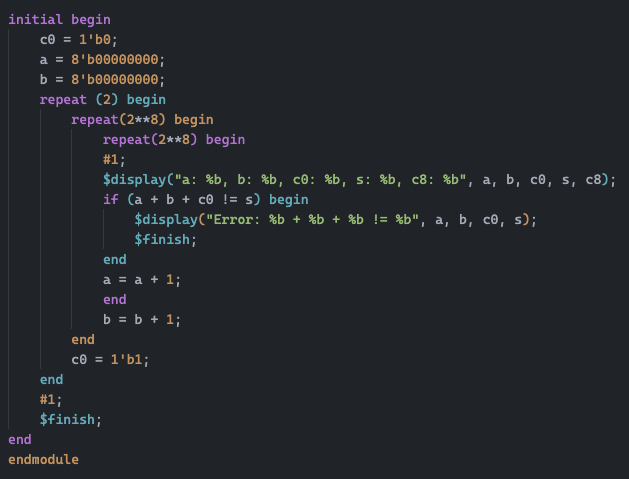
\includegraphics[width=0.6\textwidth]{Q3-tb.png}
  \caption{Q3 testbench code}
  \label{fig:Q3_tb}
\end{figure}

\begin{figure}[htp]
  \centering
  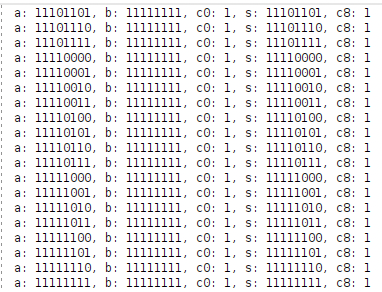
\includegraphics[width=0.5\textwidth]{Q3-display.png}
  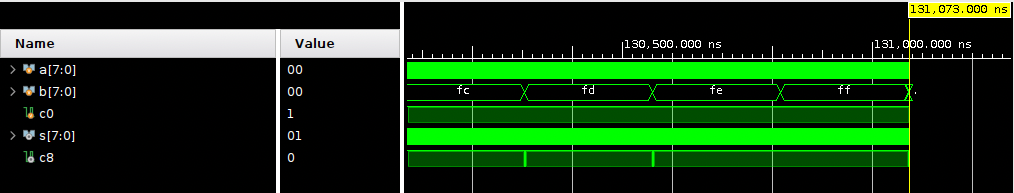
\includegraphics[width=\textwidth]{Q3-wave.png}
  \caption{Q3 testbench results}
  \label{fig:Q3_wave}
\end{figure}

\newpage

\section{Q4: 4-bit multiplier}

這個題目要完成一個 4-bit 的乘法器,透過兩個 4-bit 相乘得到一個 8-bit 的結果。
\par
根據直式乘法,可以發現一個 4-bit 乘法可以被分為四個階段,每個階段的輸出皆會往左平移一位,\
導致了四個階段的結果並不能直接對齊。
\par
但我們能夠將所有空缺的地方,補上 $0$,如此一來四個階段的結果便是對齊的四個 8-bit 數字,\ 
再將這四個結果透過章節 \ref{sec:Q3} 的 CLA 進行加法即可算出答案,電路圖如 \ref{fig:Q4_circuit}。

\begin{table}[htp]
  \centering
  \[
    \begin{array}{r r r r r r r r r r}
      & & & & & a_3 & a_2 & a_1 & a_0 \\
      & & & & \times & b_3 & b_2 & b_1 & b_0 \\
      \cline{5-9}
      & 0 & 0 & 0 & 0 & a_3b_0 & a_2b_0 & a_1b_0 & a_0b_0 \\
      & 0 & 0 & 0 & a_3b_1 & a_2b_1 & a_1b_1 & a_0b_1 & 0 \\
      & 0 & 0 & a_3b_2 & a_2b_2 & a_1b_2 & a_0b_2 & 0 & 0 \\
      + & 0 & a_3b_3 & a_2b_3 & a_1b_3 & a_0b_3 & 0 & 0 & 0 \\
      \cline{1-9}
      & p_7 & p_6 & p_5 & p_4 & p_3 & p_2 & p_1 & p_0 \\
    \end{array}
    \]
  \caption{4-bit multiplier}
  \label{tab:polynomial-multiplication}
  \end{table}
  \begin{figure}[h]
    \centering
    \includegraphics[width=\textwidth]{Q4-circuit.png}
    \caption{4-bit multiplier circuit}
    \label{fig:Q4_circuit}
  \end{figure}


\newpage

\subsection{Testbench}


枚舉 $a, b$ 的 $2^4 \times 2^4$ 種情況,並使用 display 與 if 判斷式來確認結果是否正確\
執行的一部分結果如圖 \ref{fig:Q4_display}。

\begin{figure}[htp]
  \centering
  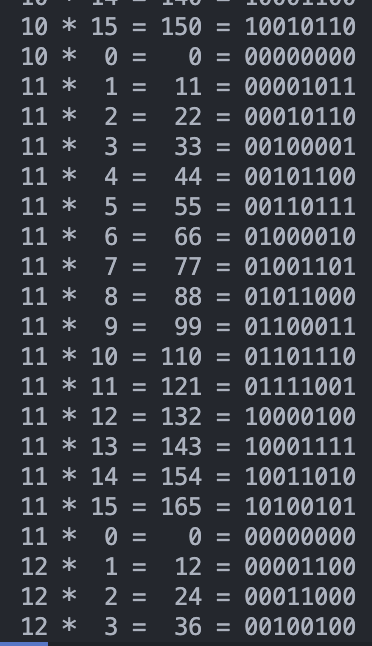
\includegraphics[width=0.2\textwidth]{Q4-display.png}
  \caption{Q4 testbench display}
  \label{fig:Q4_display}
\end{figure}

\newpage

\section{Q5: Exhausitive test}
這部分需要我們寫一個能夠涵蓋所有狀況的 Testbench,並且輸出的 $error, done$ bit 以下圖的方式呈現:
\begin{figure}[h]
  \centering
  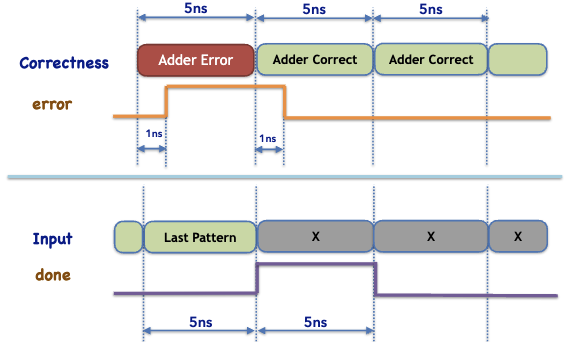
\includegraphics[width=0.6\textwidth]{Q5-spec.png}
  \caption{Q5 spec}
\end{figure}

\newpage
\subsection{Implement}
\subsubsection*{枚舉所有情況:}
這個 Testbench 有 3 個可調參數:$a, b, cin$,如果我們需要測試所有可能的情況,最簡單的方式便是利用枚舉找出所有狀態。
\par
因此我們透過三層的 repeat 迴圈,分別枚舉 $cin = [0, 1], a = [0, 2^4-1], b = [0, 2^4 - 1]$\ 

\subsubsection*{確認結果:}
接著由於題目要求,以及確保輸出是參數調整過後的,在迴圈開始後先延遲了一單位的時間,\
接著透過 display 指令輸出目前的參數以及結果以利觀察,最後再透過 if 判斷式確認 $sum$ \
是否 $= cin + a + b$,即可判斷出是否有錯誤。

\subsubsection*{error:}
根據題目要求,$error$ 訊號需要延遲 1ns,因此我們將 error bit 的設定放置於上面提到的,\
if 判斷式之中。

\subsubsection*{done:}
由於題目要求在測試結束後將 $done$ 訊號設為 True 5ns,因此在枚舉結束後將 $done$ 設為 True,\
5ns 過後再將其重設為 False。

\subsection{Wave}

根據題目要求,在模擬結束後,需要將 $done$ 設為 True 5ns。\
實作呈現如圖 \ref{fig:Q5_wave1}。

\begin{figure}[htp]
  \centering
  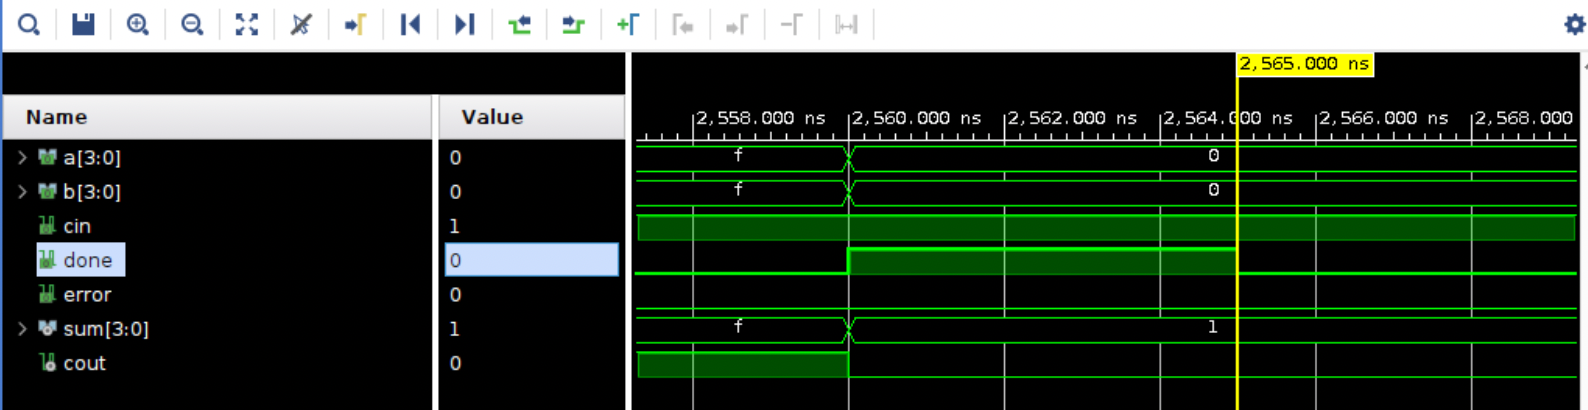
\includegraphics[width=0.8\textwidth]{Q5-wave1.png}
  \caption{Q5 testbench wave-done}
  \label{fig:Q5_wave1}
\end{figure}

根據題目要求,當錯誤發生時,需要將 $error$ 設為 True,並帶有 1ns 的延遲\
實作呈現如圖 \ref{fig:Q5_wave2}。\ 

\begin{figure}[htp]
  \centering
  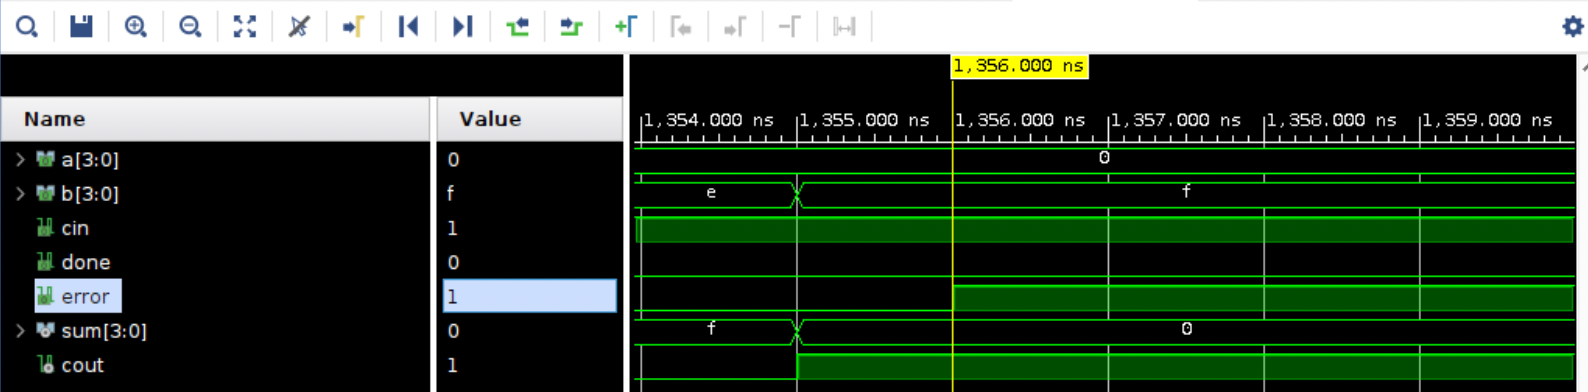
\includegraphics[width=0.8\textwidth]{Q5-wave2.png}
  \caption{Q5 testbench wave-error}
  \label{fig:Q5_wave2}
\end{figure}

\newpage

\section{Q6: FPGA display Control}
最後則是要將 \ref{sec:Q2} 的結果,透過 FPGA 上開關作為訊號表示,並將結果由七段顯示器顯示出來。

\subsection{Implement}
我們定義了一個 module: Display\_Control,輸入 $rs, rt, sel$ 並輸出 $seg, an$。\ 
\par
連接章節 \ref{sec:Q2} 的 module,得到 $rd$ 之後,建立 $16$ 條線,\
透過 AND $rd$ 讓相對應的線變成 True,而其他的為 False。
\par
最後一步是判斷七段顯示器中 $A \sim G$ 七個燈條哪些要亮,根據簡單的統計,可以得到每個燈條在哪些數字需要亮:\
($10 \sim 15$ 將顯示為:A, b, C, d, E, F, G),實作程式碼如圖 \ref{fig:SymbolA}。
\begin{enumerate}
  \item $A: 0, 2, 3, 5, 6, 7, 8, 12, 14, 15$
  \item $B: 0, 1, 2, 3, 4, 7, 8, 9, 10, 13$
  \item $C: 0, 1, 3, 4, 5, 6, 7, 8, 9, 10, 11, 13$
  \item $D: 0, 2, 3, 5, 6, 8, 11, 12, 13, 14$
  \item $E: 0, 1, 6, 8, 10, 11, 12, 13, 14, 15$
  \item $F: 0, 4, 5, 6, 8, 9, 10, 11, 12, 14, 15$
  \item $G: 2, 3, 4, 5, 6, 8, 9, 10, 11, 13, 14, 15$ 
\end{enumerate}

\begin{figure}[h]
    \centering
    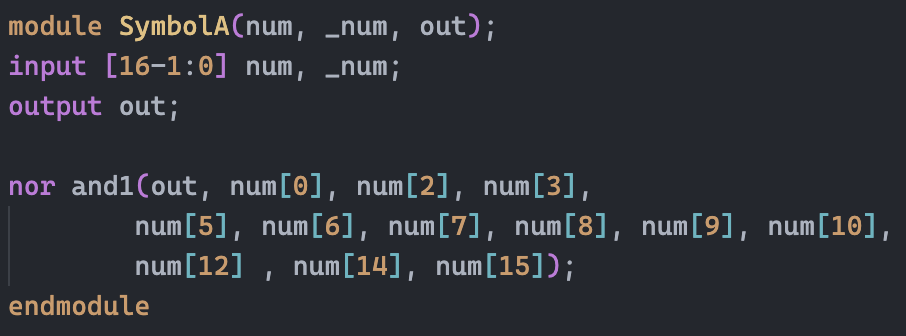
\includegraphics[width=0.8\textwidth]{SymbolA.png}
    \caption{Symbol A code}
    \label{fig:SymbolA}
\end{figure}

由於 FPGA 上是當訊號為 False 時,燈條會亮,因此我們只需要將上述的數字做 nor 運算,即可得到每個燈條的訊號。

至於 $an$ 因為是固定只顯示一個數字,因此就直接使用 AND 設定成 $1110_{(2)}$ 即可。


最後將 $seg, an$ 依照 FPGA 上的 Port 設定 IO,便完成了 Display Control 的設計,\ 
實際運行將會在上機時演示。

\newpage
\section{Other}

\subsection{我們學到了什麼}
\subsubsection*{Decode and execute}
寫完這個題目之後發現,這其實就是 CPU 中接收機器碼並運算的核心概念,\
只要有辦法使其擴充並支援某個指令集,便可以完成一個簡單的運算單元。
\par
在完成這個作業之後,我去瞭解了一下 RISC-V 的指令集架構,發現由於是精簡指令集,\
Instruction 數量基本上是在能夠實作的範圍內,因此單純運算單元應該是有辦法實現的。\
但因為 FPGA 的存儲空間有限,因此最大的問題在於如何實現 memory controler,\
這也是我們在接下來的課程中要去嘗試想像的。

\subsubsection*{不同指令之間的速度差異}
在撰寫程式時,經常可以發現同樣的結果、時間複雜度,使用不同運算子的速度差異頗大,\
雖然可以想像其原因,不過真正實作過後才能真的感受到這個差異。

\subsubsection*{七段顯示器}
FPGA 七段顯示器的 IO,分為兩個部分,一個是 $an$,另一個是 $seg$,\
分別代表要亮哪個數字,以及要亮那個數字中的哪幾顆 LED 燈。可以發現到,\
不同數字之間的 $seg$ 是共用的,讓我學到了原來七段顯示器是透過不斷了輪流亮燈,\
利用人眼的是視覺暫留來達到顯示多個數字的效果。

\subsection{分工}
\begin{itemize}
  \item 陳克盈:程式碼、報告撰寫,蔡明妡:電路圖
\end{itemize}

\end{document}


